%%Designed for IEEE Transactions on Vehicular Technology, based on bare_jrnl.tex by Michael Shell.
%%December. 2015
%%Length Requirements: The complete manuscript  should be prepared in final IEEE typesetting with maximum page length limited to 15 pages for a Regular Paper and 5 pages  for a Correspondence. 
%%Contact Info: admin-tvt@ece.ufl.edu
%%Designed by TVT editorial office


\documentclass[journal,10pt]{IEEEtran}
\usepackage[numbers,sort&compress]{natbib}
\usepackage{dsfont}
\usepackage{amssymb}
\usepackage{graphicx}
\usepackage{epsfig}
\usepackage{CJK}
\usepackage{amsmath}
\usepackage{multirow}
\usepackage{subfigure}

\begin{document}
\bibliographystyle{IEEEtran}
\title{Cellular System Performance Analysis Under Correlated Shadow Fading}


\author{Tingting~Lu,~\IEEEmembership{Student~Member,~IEEE,}
        Pei~Liu,~\IEEEmembership{Member,~IEEE,}
        and~Shivendra~S.~Panwar,~\IEEEmembership{Fellow,~IEEE}% <-this % stops a space

\thanks{The authors are with the Department of Electrical and Computer Engineering, Tandon Engineering School of New York University, Brooklyn, NY, 11201}% <-this % stops a space
\thanks{Manuscript received XXX, XX, 2017; revised XXX, XX, 2017.}}

\markboth{IEEE Transactions on Vehicular Technology,~Vol.~XX, No.~XX, XXX~2017}
{}
%{Shell \MakeLowercase{\textit{et al.}}: Bare Demo of IEEEtran.cls for Journals}







\maketitle
\begin{abstract}
In a cellular network, connections between the Base Station (BS) and Mobile Stations (MSs) may be disrupted when the channel has low signal-to-interference-plus-noise ratio (SINR). Shadow fading is a large-scale fading which can significantly affect signal strength and reduce SINR over a wide area. Empirical measurements show that shadowing has significant correlations in realistic scenarios that can affect system performance.  Shadow fading could result in long-lasting outage for stationary and mobile users, which will lead to flickering connections and consecutive packet losses. Such a link is especially harmful to real-time applications that are delay sensitive. Increasing diversity of the system is considered a way to increase SINR. Therefore, increasing the BS density and allow users to connect to multiple BSs can help to reduce the number of long-lasting outage durations, and provide better Quality of Service (QoS) support for delay sensitive applications. This paper focuses on a study of the downlink performance of a multi-cell communication system under correlated shadow fading. The outage probability of a grid layout and a random layout of BSs are presented. First, we compare the outage probability of the two different BS layout models with similiar correlated shadow fading. Simulation results indicate that the grid model has better performance than the random model. Secondly, the outage probability with independent shadow fading and correlated shadow fading for the random BS layout is demonstrated. Thirdly, we focus on the more realistic random BS model, and present the distribution of outage durations given independent shadow fading or correlated shadow fading. Simulation results demonstrate that outage durations with correlated shadow fading are longer than those with the independent shadow fading. At the end, we show that increasing the BS density can mitigate the effect of correlated shadow fading and improve the system performance by reducing the outage durations. 

\end{abstract}


\begin{IEEEkeywords}
Correlated shadow fading, outage probability, outage duration.
\end{IEEEkeywords}

\section{Introduction and Related Works}
\begin{figure}
\centering
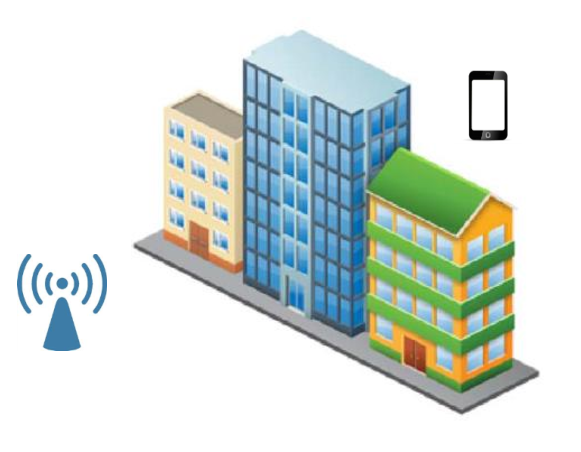
\includegraphics[width=6cm]{building.eps}
\caption{An example of building blockage.}
\label{building}
\end{figure}
\par In a cellular communication system, the connection between a BS and a MS may be dropped when the MS enters a deep fading area. Fading phenomena can substantially affect the performance of a wireless communication system. In general, fading can be divided into two categories: large-scale fading and small-scale fading. A signal transmitted from source to destination will experience both large-scale and small-scale fading. Small-scale fading is caused by multipath propagation. Large-scale fading, which is also known as shadow fading, is caused by obstacles (trees, buildings, etc.) in the propagation path. In most cases, shadow fading is assumed to be temporally and spatially independent \cite{rappaport1996wireless}.  However, researchers have also shown that shadow fading is spatially correlated at different positions on the propagation path \cite{gudmundson1991correlation}, \cite{zhang2008novel}. In \cite{fabbri2009impact} and \cite{patwari2008effects}, the effects of correlated shadowing in connectivity is demonstrated, which indicates that reliable connectivity will be much more difficult to maintain than indicated by independent shadow fading models. The spatial correlation of shadow fading is important when studying the QoS of a mobile system since it will result in long-lasting outage durations, which will deteriorate the performance of the applications running on the network. For example, in Fig. \ref{building}, the MS is moving behind a row of tall buildings which block the signals from the BS. These tall buildings result in deep shadow fading, and the shadow fading of different positions behind these buildings are closely correlated. To investigate the system performance under correlated shadow fading, this paper focuses on outage probability and outage duration analysis under correlated shadow fading in a multi-cell communication system. Based on the analysis, we provide a solution to reduce the frequency and duration of dropped connections.

\par There have been a lot of studies on the outage probability of cellular communication systems \cite{abu1991outage, petrovic2013outage, emamian2014outage}. The author of \cite{vural2015effect} analyzed the outage probability and the coverage area under independent shadow fading, which follows Log-normal distribution, Weibull distribution and Gamma distribution. In contrast, there is much less work on the outage probability and outage duration, given the correlations in shadow fading. Consequently, performance of a multi-cell system with correlated shadow fading remains an open problem. In \cite{lu2015long} and \cite{lu2015shining}, we discussed the outage probability and the outage duration distribution of a single-cell communication system under the exponentially correlated shadow fading and the distance-angle correlated shadow fading. For a single-cell model, exponentially correlated shadow fading can be modeled as a Markov chain model. Highly correlated shadow fading will result in long-lasting outage durations. In \cite{lu2015shining}, a single-cell model under the distance-angle correlated shadow fading is investigated. Correlated shadow fading leads to correlated outage events and long-lasting outage durations. To overcome these disadvantages, we propose a cooperative communication scheme to mitigate shadow fading by deploying relays at the cell edge. \cite{lu2015long} and \cite{lu2015shining} are limited to the single-cell model. In this paper, we are going to extend the study to review the impact of correlated shadow fading on a multi-cell model, and provide a solution to overcome the long-lasting outage durations.
\par For the multi-cell system, a new general model for the user SINR was developed using stochastic geometry \cite{andrews2011tractable}. The cellular network was modeled by placing BSs at locations as a homogeneous Poisson Point Process (PPP). The author concluded that, under general fading, increasing the number of BS did not affect the coverage probability and/or the outage probability, as long as the MS was connecting to the nearest BS. Moreover, the paper did a comparison between the grid model and the PPP model, and concluded that the regular grid model provided the upper bound of the coverage probability while the PPP model provided the lower bound. The authors also considered the effect of independent log-normal interference, and concluded that, higher log-normal interference increases coverage probability, which seems counter-intuitive. The author explained that increasing randomness gave the cell edge users, which have poor mean SINR, an increasing chance of being in coverage. However, the author did not consider the scenario with correlated log-normal shadow fading. 
\par A comparative analysis of the random topology and the grid topology of a small cell network deployment was given in \cite{chen2012small}. In this paper, the spatial outage probability and the spatial average throughput, versus the number of access points of the two different network deployments were illustrated under independent shadow fading. Approximating the outage probability and the capacity for $\kappa-\mu$ shadow fading was discussed in \cite{kumar2015approximate}. $\kappa-\mu$ shadow fading includes the one-sided Gaussian, the Rayleigh, the Nakagami-m and the Rician. As we mentioned before, the empirical shadow fading measurements did not exhibit such features. Therefore, those complex features are not the main focus when investigating system performance under correlated shadow fading.
\par In most cases, shadow fading is modeled as an independent log-normal distribution \cite{goldsmith2005wireless} with a standard deviation derived from empirical measurements. An independent log-normal shadowing model is used widely when shadow fading cannot be ignored. In the log-normal shadowing model, the path loss $\psi$ is assumed random, with a log-normal distribution given by
\begin{equation}
p(\psi)=\frac{\xi}{\sqrt{2\pi}\sigma_{\psi_{dB}}\psi}exp[-\frac{(10\log_{10}\psi-\mu_{\psi_{dB}})^{2}}{2\sigma_{\psi_{dB}}^{2}}], \psi>0,
\end{equation}
where $\xi=10/\ln10$, $\mu_{\psi_{dB}}$ is the mean of $\psi_{dB}=10\log_{10}\psi$ and $\sigma_{\psi_{dB}}$ is the standard deviation of $\psi_{dB}$.
The distribution of the $dB$ value of $\psi$ is Gaussian with mean $\mu_{\psi_{dB}}$, standard deviation $\sigma_{\psi_{dB}}$ and is given by:
\begin{equation}
p(\psi_{dB})=\frac{1}{\sqrt{2\pi}\sigma_{\psi_{dB}}}exp[-\frac{(\psi_{dB}-\mu_{\psi_{dB})^2}}{2\sigma_{\psi_{dB}}^2}].
\end{equation}
The above model fails to capture the spatial correlations in shadow fading. Empirical measurements show that shadowing has significant correlations in realistic scenarios that can affect system performance \cite{graziano1978propagation}. Considering the distribution of obstructions and the speed of the MS, a realistic channel propagation model should incorporate correlated shadow fading.  Szyszkowicz et al. \cite{szyszkowicz2010feasibility} presented a review and analysis of the feasibility of different correlated shadowing models. For a multi-cell model with multiple BSs at different places, both autocorrelation and cross-correlation need to be taken care of. To simplify the simulation, the exponential correlation model is chosen in this paper.



 \par The key contributions of this paper are summarized as follows:
 \begin{itemize}
 \item Analyze the relationship between correlated shadow fading and correlated outage events under correlated outage fields.
 \item Investigate the outage probability of both the Grid model and the Random model given correlated shadow fading.
 \item Illustrate how increasing the BS density helps mitigate the correlated shadow fading for the Random model in terms of reducing the outage probability (coverage probability) and the percentage of long-lasting outage durations.
 \item Analyze the relation between the tunable parameter (de-correlation distance) of the correlated shadow fading model and the outage probability.
 \item Compare the performance of the system with regard to different MS-BS connection strategies: MS connecting to the nearest BS versus MS connecting to the BS providing the strongest signal.
 \end{itemize}
 The paper is organized as follows: Section \ref{CorrShadowField} presents the correlated shadow fading model used in this paper and the resultant correlated outage field. Section \ref{SystemModel} illustrates the system model with two different BS deployments and investigates the outage probability given the two deployments. Section \ref{OutageProb} gives a theoretical analysis of the outage probability given correlated shadow fading. Section \ref{4:SimuProb} presents the simulation setup and analyzes the simulation results from different BS densities. Section \ref{Conclusion} summarizes the paper and proposes future work directions.

\section{Correlated Shadow Fading}
\label{CorrShadowField}
As stated in the introduction, empirical measurements show that there exist different patterns of correlations between the shadowing. The independent log-normal shadow fading model, while is very useful for static MS performance analysis, cannot reflect the correlation of shadow fading between different locations. In this section, we will give a brief introduction of shadow fading models, including the model used in this paper.
In most cases, shadow fading is considered as independent log-normal. But from empirical measurements we can conclude that there exit different correlations between shadow fading factors. There is no single mathematical model which captures all different categories of correlation\cite{szyszkowicz2010feasibility}. In this paper, we use the most commonly used exponentially correlated shadow fading model \cite{szyszkowicz2011interference}. In \cite{szyszkowicz2011interference}, the author states that correlation in shadowing is indispensable for the analysis of interference of large networks. An exponentially correlated shadowing field $S$ with shadow fading factor $s_{i}$ for each position $p_{i}$ has a correlation matrix as below:
\begin{equation}
\mathbf{K}_{N\times N} = [ \sigma_{s}(p_{i})\sigma_{s}(p_{j})\rho(i,j)],
\label{correlationmatrix}
\end{equation}
where $N$ is the length of the shadowing field. Suppose $A$ and $B$ are two neighboring points, the shadow fading (in dB) is $N(0,\sigma^2)$ where $\sigma$ is the standard deviation. The spatial correlation between $s_{A}$ and $s_{B}$ will be given by 
\begin{equation}
\rho_{A,B} = \frac{E[s_{A}s_{B}]}{\sigma^2} =e^{-\frac{d_{A,B}}{d_{0}}}
\end{equation}
where $d_{0}$ is de-correlation distance and  $d_{A, B}$ denotes the distance between $A$ and $B$.
\begin{figure}
\centering
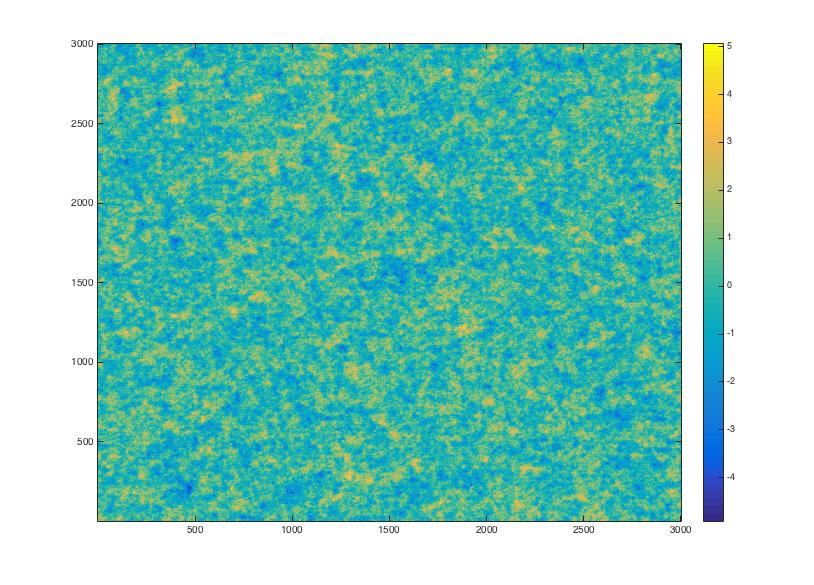
\includegraphics[width = 8cm]{ShadowFieldDeCorr20.jpg}
\caption{Exponentially correlated shadowing field with $d_{0} = 20m$ (the color of the area refers to the normalized standard deviation  which is $S_{i}/\sigma_{s}(i)$)}

\label{shadowingfield}
\end{figure}
Follow the shadowing field generation algorithm, we generate shadowing fields with different  de-correlation distances. A sample correlated shadowing field is shown in Fig. \ref{shadowingfield}. In Fig. \ref{shadowingfield}, deeper color means deeper fading. Deep blue colors are aggregating together to show the pattern of correlation. When the MS gets into the blue region (deep fading region), it will stay in that region for a certain period of time. Due to this correlation, a MS in deep fading area may experience long-lasting outage duration.
\par Given a correlated shadowing field, the outage events at different locations are correlated. Without considering small-scale fading, the channel gain at different locations has a spatial correlation. An outage event occurs when SINR becomes less than $\gamma$, where $\gamma$ is a given SINR threshold. Based on the aforementioned correlated shadow fading model and the Random model in section \ref{SystemModel}, a correlated outage field can be generated as in Fig. \ref{4:outagefie}. On the left, an outage field with independent log-normal shadow fading is shown, while the correlated outage field with correlated shadow fading is given on the right. The black color indicates outage areas. Outage areas due to the independent shadow fading are uncorrelated dots. In contrast, those under the correlated shadow fading contain several connected areas . Therefore, we conclude that correlated shadow fading results in correlated outage areas.

 \begin{figure*}
 \centering
 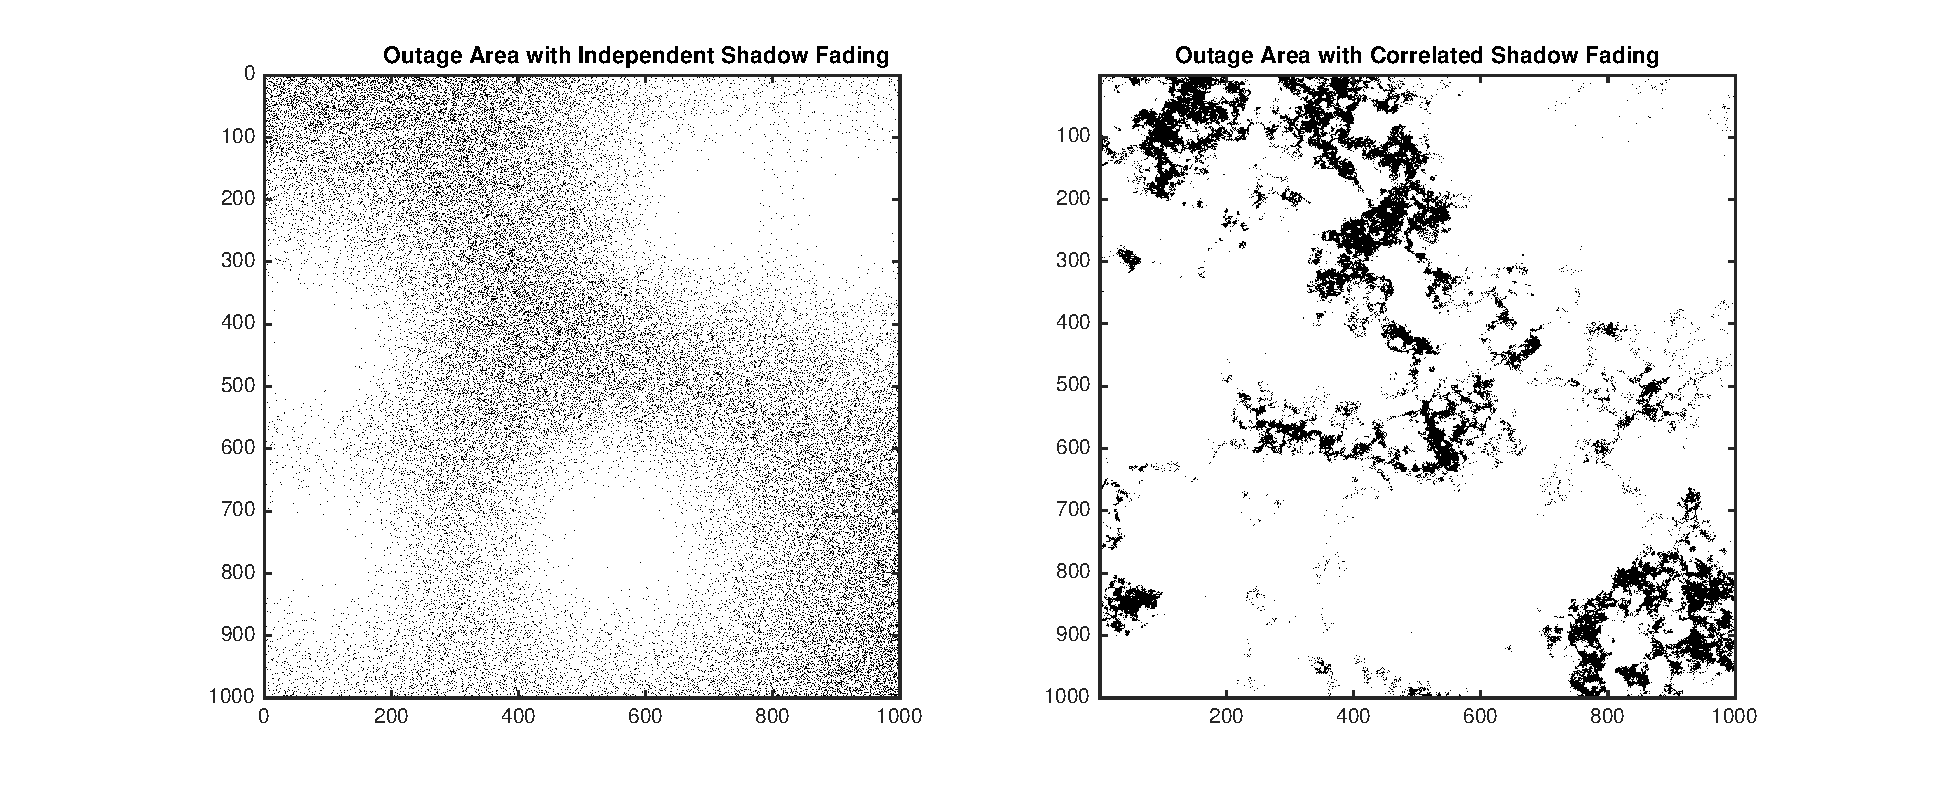
\includegraphics[width=14cm]{outageArea.eps}
 \caption{Correlated outage fields (Dark areas are outage areas while white areas are non-outage areas)}
 \label{4:outagefie}
 \end{figure*}
 \section{System Model}
 \label{SystemModel}
 In this section, we consider two system models with two different BS deployments: the Grid model and the Random model.
 \begin{itemize}
 \item Grid model: $\lambda$ BSs are placed on a regular grid deterministically.
 \item Random model: $\lambda$ BSs are placed randomly in a fixed area.
 \end{itemize}
 \begin{figure}
 \centering
 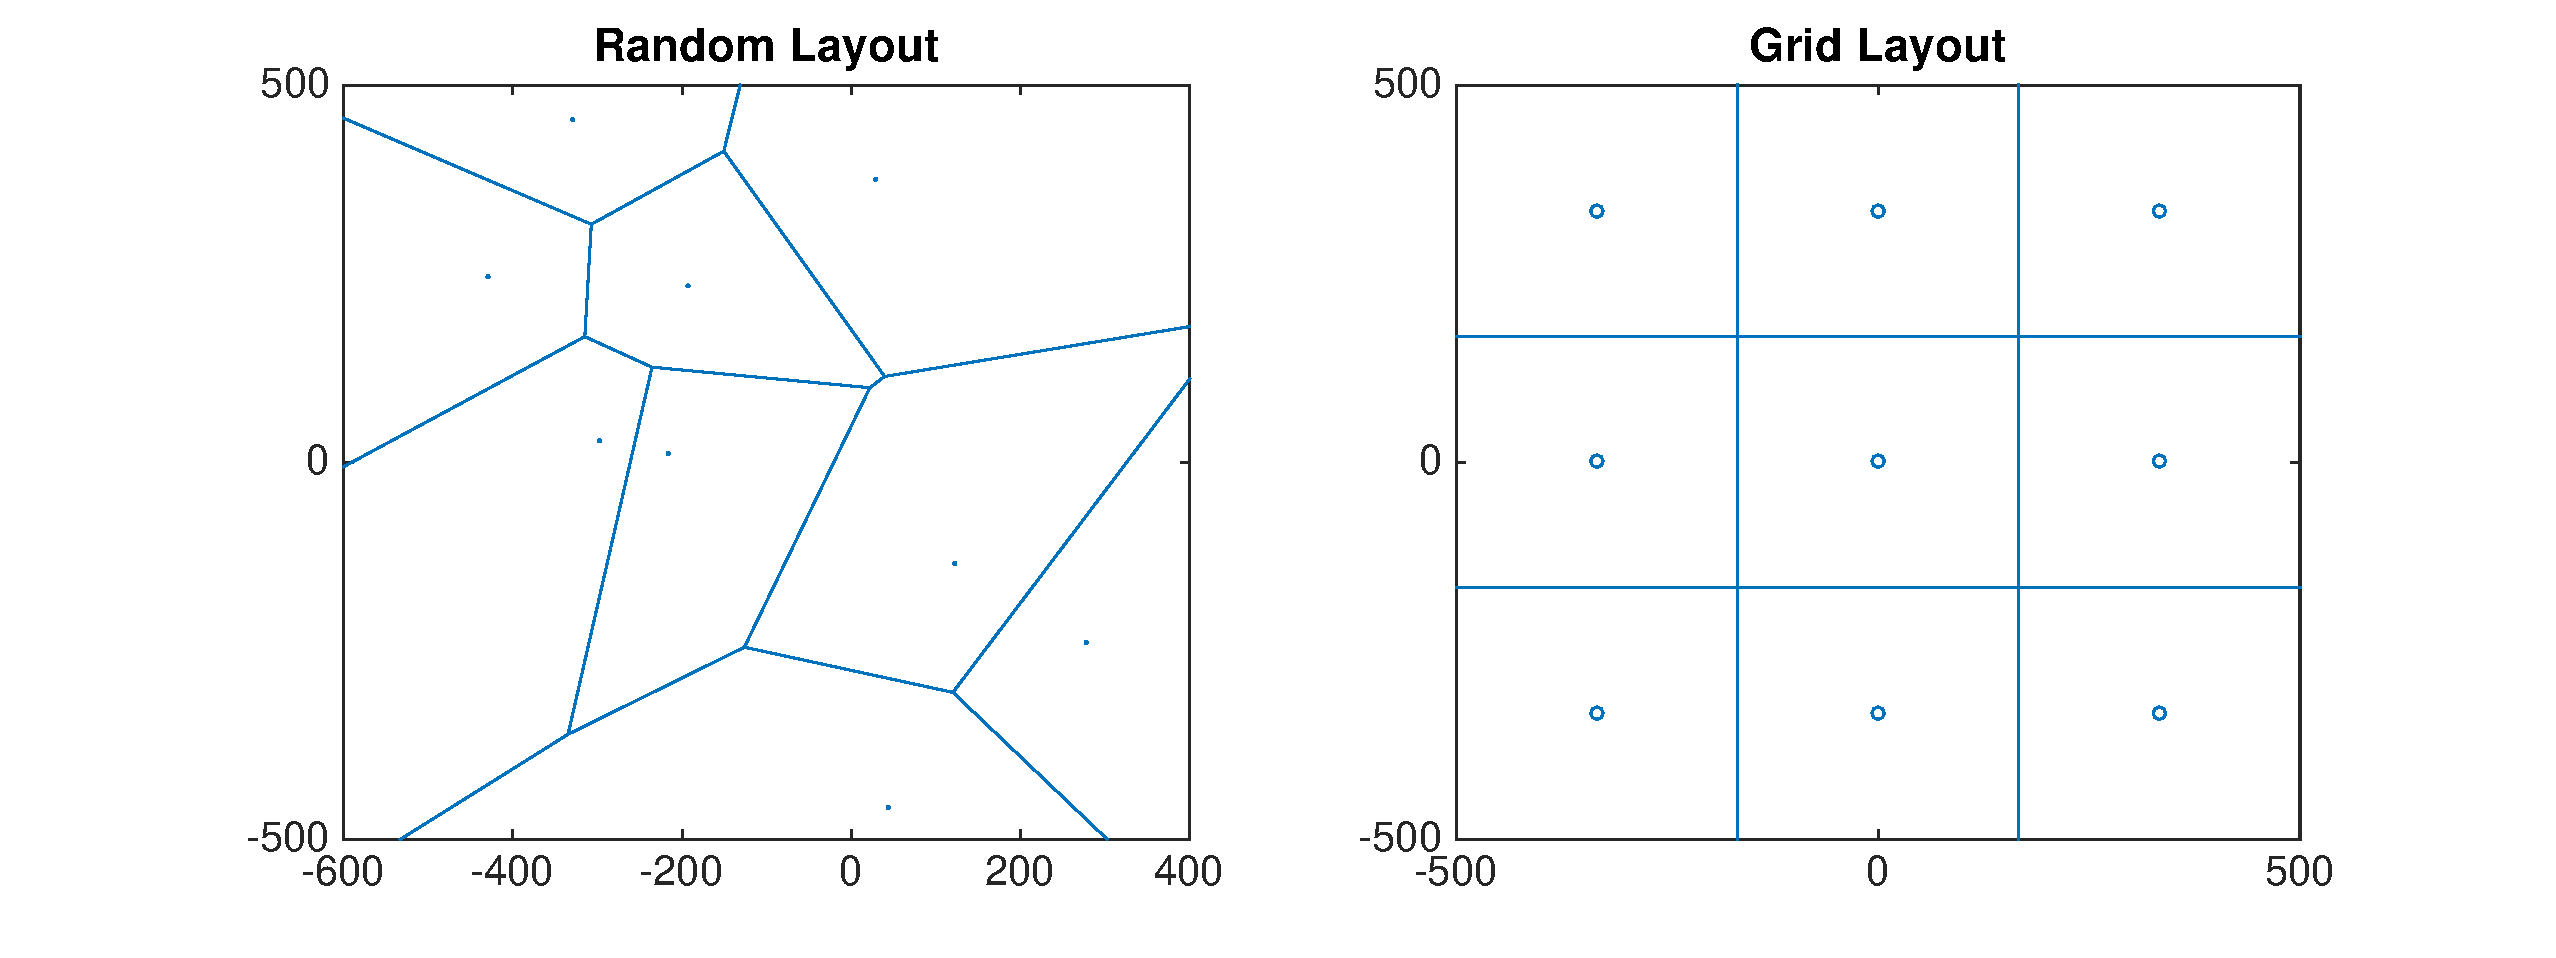
\includegraphics[width=9cm]{systemLayout.eps}
 \caption{Random model and Grid model with $\lambda = 9$.}
 \label{4:RandomLayout}
 \end{figure}
 % \begin{figure}
 % \centering
 % \includegraphics[width=8cm]{GridLayout.eps}
 % \caption{Grid Base Station Locations}
 % \label{GridLayout}
 % \end{figure}
On the left of Fig. \ref{4:RandomLayout}, an example of the grid model is presented, where cells are square shaped and of the same size. For the Random model shown on the right, cells are not guaranteed to be the same shape or the same size. Distances between nearest base stations have a large variation from cell to cell.


 \section{Outage Probability Analysis}
 \label{OutageProb}
 \par Let $\varphi = \{1, 2, \dots, N\}$ denote the set of all BSs, then the received signal from BS $i$ to the destination user $D$ is given by:
 \begin{equation}
 y_{i\to D} = G_{i\to D}x_{i}+n_{D}.
 \end{equation}
 where $x_{i}$ is the signal transmitted by the source BS and $y_{i\to D}$ is the signal received by the destination user. $n_{D}\sim \mathcal{CN}(0,N_{0})$ is additive white Gaussian noise. $G_{i\to D}$ is the channel gain from source BS to MS including path loss and shadow fading. The end-to-end received $\text{SINR}$ is given below:
 \begin{equation}
 \text{SINR} \triangleq \frac{P_{i}*G_{i\to D}^{2}}{N_{0}+\sum_{j\in \varphi/i}P_{j}*G_{j\to D}^2},
 \end{equation}
 where $P_{i}$ is the transmitted power of BS $i$. The MS successfully receives the signal if no outage event occurs, i.e., $\log_{2}(1+\text{SINR})\ge R$, where $R$ is the required data rate. From the definition of SINR, no outage event occurs as long as $\text{SINR} > \gamma$, where $\gamma = 2^{R}-1$.

 \par For a particular MS, outage event occurs when its received SINR is less than a threshold to decode the received signal. In our scenario, the probability that the receiver cannot decode signals received from its serving BS is defined as:
 \begin{equation}
 P(out_{i}) = P[\text{SINR}_{i\to D} < \gamma].
 \end{equation}
 We investigate two connection strategies: 
 \begin{itemize}
 \item Nearest BS: MS chooses to connect to the nearest BS.
 \item Strongest BS: MS chooses to connect to the BS providing highest SINR.
 \end{itemize}
 \par In the Nearest BS mode, we assume that the MS is served by the nearest BS, then the outage probability will be 
 \begin{equation}
 P_{out} = P_{out_{i}},
 \end{equation} 
 where $i$ is the index of the nearest BS. 
 \par In the Strongest BS mode, under the assumption that an MS is always connecting to the BS which provides the highest SINR, the outage event occurs if no BS can provide high enough SINR to the receiver. Based on this assumption we have:
 \begin{equation}
 P_{out} = \max_{i = 1,\cdots,N} P[\text{SINR}_{i\to D}<\gamma].
 \end{equation}
 The probability density function (pdf) of shadow fading $S$ given $L$ correlated fading branches is
 \begin{equation}
 \begin{split}
 f_{\mathbf{S}}(\mathbf{s}) = &\frac{\lambda^{L}}{\sqrt{2\pi}|\mathbf{K}_{L\times L}|^{1/2}\prod_{i=1}^{L}s_{i}}\\
 &\cdot\exp(-\frac{1}{2}(10\log_{10}\mathbf{s}-\boldsymbol{\mu})^{T}\mathbf{K}_{L\times L}^{-1}(10\log_{10}\mathbf{s}-\boldsymbol{\mu})),
 \end{split}
 \end{equation}
 where $\lambda = 10/\ln10$ and $\boldsymbol{\mu}$ is the average shadow fading which is normally $0$. $\mathbf{K}_{L\times L}$ is the correlation matrix which is defined in \eqref{correlationmatrix}. Let $\theta_{i} = \frac{10\log_{10}s_{i}-\mu_{i}}{\sqrt{2}\sigma_{i}}$, and doing a change of variables gives us the pdf of $\mathbf{\Theta}$ as follows:
 \begin{equation}
 f_{\mathbf{\Theta}}(\boldsymbol{\theta}) = \frac{1}{\pi^{L/2}|\mathbf{\Sigma}|^{1/2}}\exp(-\mathbf{\Theta}^{T}\mathbf{\Sigma}^{-1}\mathbf{\Theta}),
 \end{equation}
 where $\mathbf{\Sigma}$ is the correlation coefficient matrix which is
 \begin{equation}
 \left[\begin{array}{cccc}
 1 & h_{1,2} & \cdots & h_{1,L}\\
 \vdots & \ddots & \ddots & \vdots\\
 h_{L,1} & h_{L,2} & \cdots & 1\\
 \end{array}\right].
 \end{equation}
 Since $\text{SINR}_{i\to D}=PL_{i\to D}+S_{i}-N_{0}-\sum_{j\in\varphi/i}(PL_{j\to D} + S_{j})$ in dB, $\text{SINR}_{i\to D}<\gamma$ means
 \begin{equation}
 S_{i} - \sum_{j\in\varphi/i}S_{j}<\gamma -PL_{i\to D} + \sum_{j\in\varphi/i}PL_{j\to D} + N_{0},
 \end{equation}
 where $\varphi$ denotes the set of all BSs.
 Then the outage probability can be written as:
 \begin{equation}
 \label{4:outprob}
 P_{out} = \underbrace{\int_{-\infty}^{+\infty}\cdots\int_{-\infty}^{+\infty}}_{i =1,\cdots,N} g(PL_{i}S_{i} - \gamma\sum_{j\in\varphi/i}PL_{j}S_{j})f(\mathbf{s})d\mathbf{s},
 \end{equation}
 where $\mathbf{s}$ is the correlated shadow fading experienced by all BSs; $g(PL_{i}S_{i} - \gamma\sum_{j\in\varphi/i}PL_{j}S_{j})$ is a step function defined in (\ref{4:stepfunction}). 
  \begin{figure*}[!t]
 % ensure that we have normalsize text
 \normalsize
 % Store the current equation number.
 % \setcounter{MYtempeqncnt}{\value{equation}}
 % % Set the equation number to one less than the one
 % % desired for the first equation here.
 % % The value here will have to changed if equations
 % % are added or removed prior to the place these
 % % equations are referenced in the main text.

 \begin{equation}
 \label{4:stepfunction}
 g(PL_{i}S_{i} - \gamma\sum_{j\in\varphi/i}PL_{j}S_{j}) = \{\begin{array}{cc}
                1, &  \text{  when }PL_{i}S_{i} - \gamma\sum_{j\in\varphi/i}PL_{j}S_{j} <\frac{\gamma N_{0}}{P}\\
                0, & \text{  when }PL_{i}S_{i} - \gamma\sum_{j\in\varphi/i}PL_{j}S_{j} >\frac{\gamma N_{0}}{P}
              \end{array}.
 \end{equation}
 % Restore the current equation number.
 % \setcounter{equation}{\value{MYtempeqncnt}}
 % IEEE uses as a separator
 \hrulefill
 % The spacer can be tweaked to stop underfull vboxes.
 \vspace*{4pt}
 \end{figure*}

 \section{Simulation Results}
 \label{4:SimuProb}
 \par In this section, we present the simulation setup and results. Firstly, we execute simulations to compare the outage probability of the two different network topologies: the Grid model and the Random model. Secondly, the SINR distribution and the outage probability of the Random model given different BS densities are investigated. Two scenarios are considered: MS connecting to the nearest BS and MS connecting to the BS providing highest SINR. At the end, the outage duration distribution is simulated and discussed given different BS densities. The simulation parameters are presented in Table \ref{SystemConfig2}. 
 \begin{table}
 \centering
 \caption{\label{SystemConfig2}Simulation Configuration Parameters}

 \begin{tabular}{|c|c|}

 \hline
 Target Area & $1000m\times 1000m$\\
 \hline
 BS Densities & $3, 10, 50, 100, 200, 300, 500$\\
 \hline
 Path Loss Exponent & $4$\\
 \hline
 BS Transmission Power & $P: 40dbm$\\
 \hline
 SINR Requirement & $-5dB$\\
 \hline
 De-Correlation Distance & $20m, 200m$\\
 \hline
 \end{tabular}

 \end{table}

 \par We employ Monte-Carlo simulation to calculate the probability distribution of SINR. To start the simulation, a large number of correlated shadowing fields are generated. BSs and the MS are placed over the correlated shadow fading field. Fig. \ref{4:cdf1} shows the Cumulative Distribution Function (CDF) of SINR when the MS is connecting to the nearest BS. The de-correlation distance of the correlated shadow fading is $20m$. The figure suggests that the Grid model outperforms the Random model, which is consistent with findings in \cite{andrews2011tractable}. Fig. \ref{4:outage1} shows the outage probability with SINR threshold being $-5dB$. The outage probability of the Grid model (blue) is lower than that of the Random model (yellow). In the next section, we will focus on the Random model, which is more realistic than the Grid model.
 \begin{figure}
 \centering
 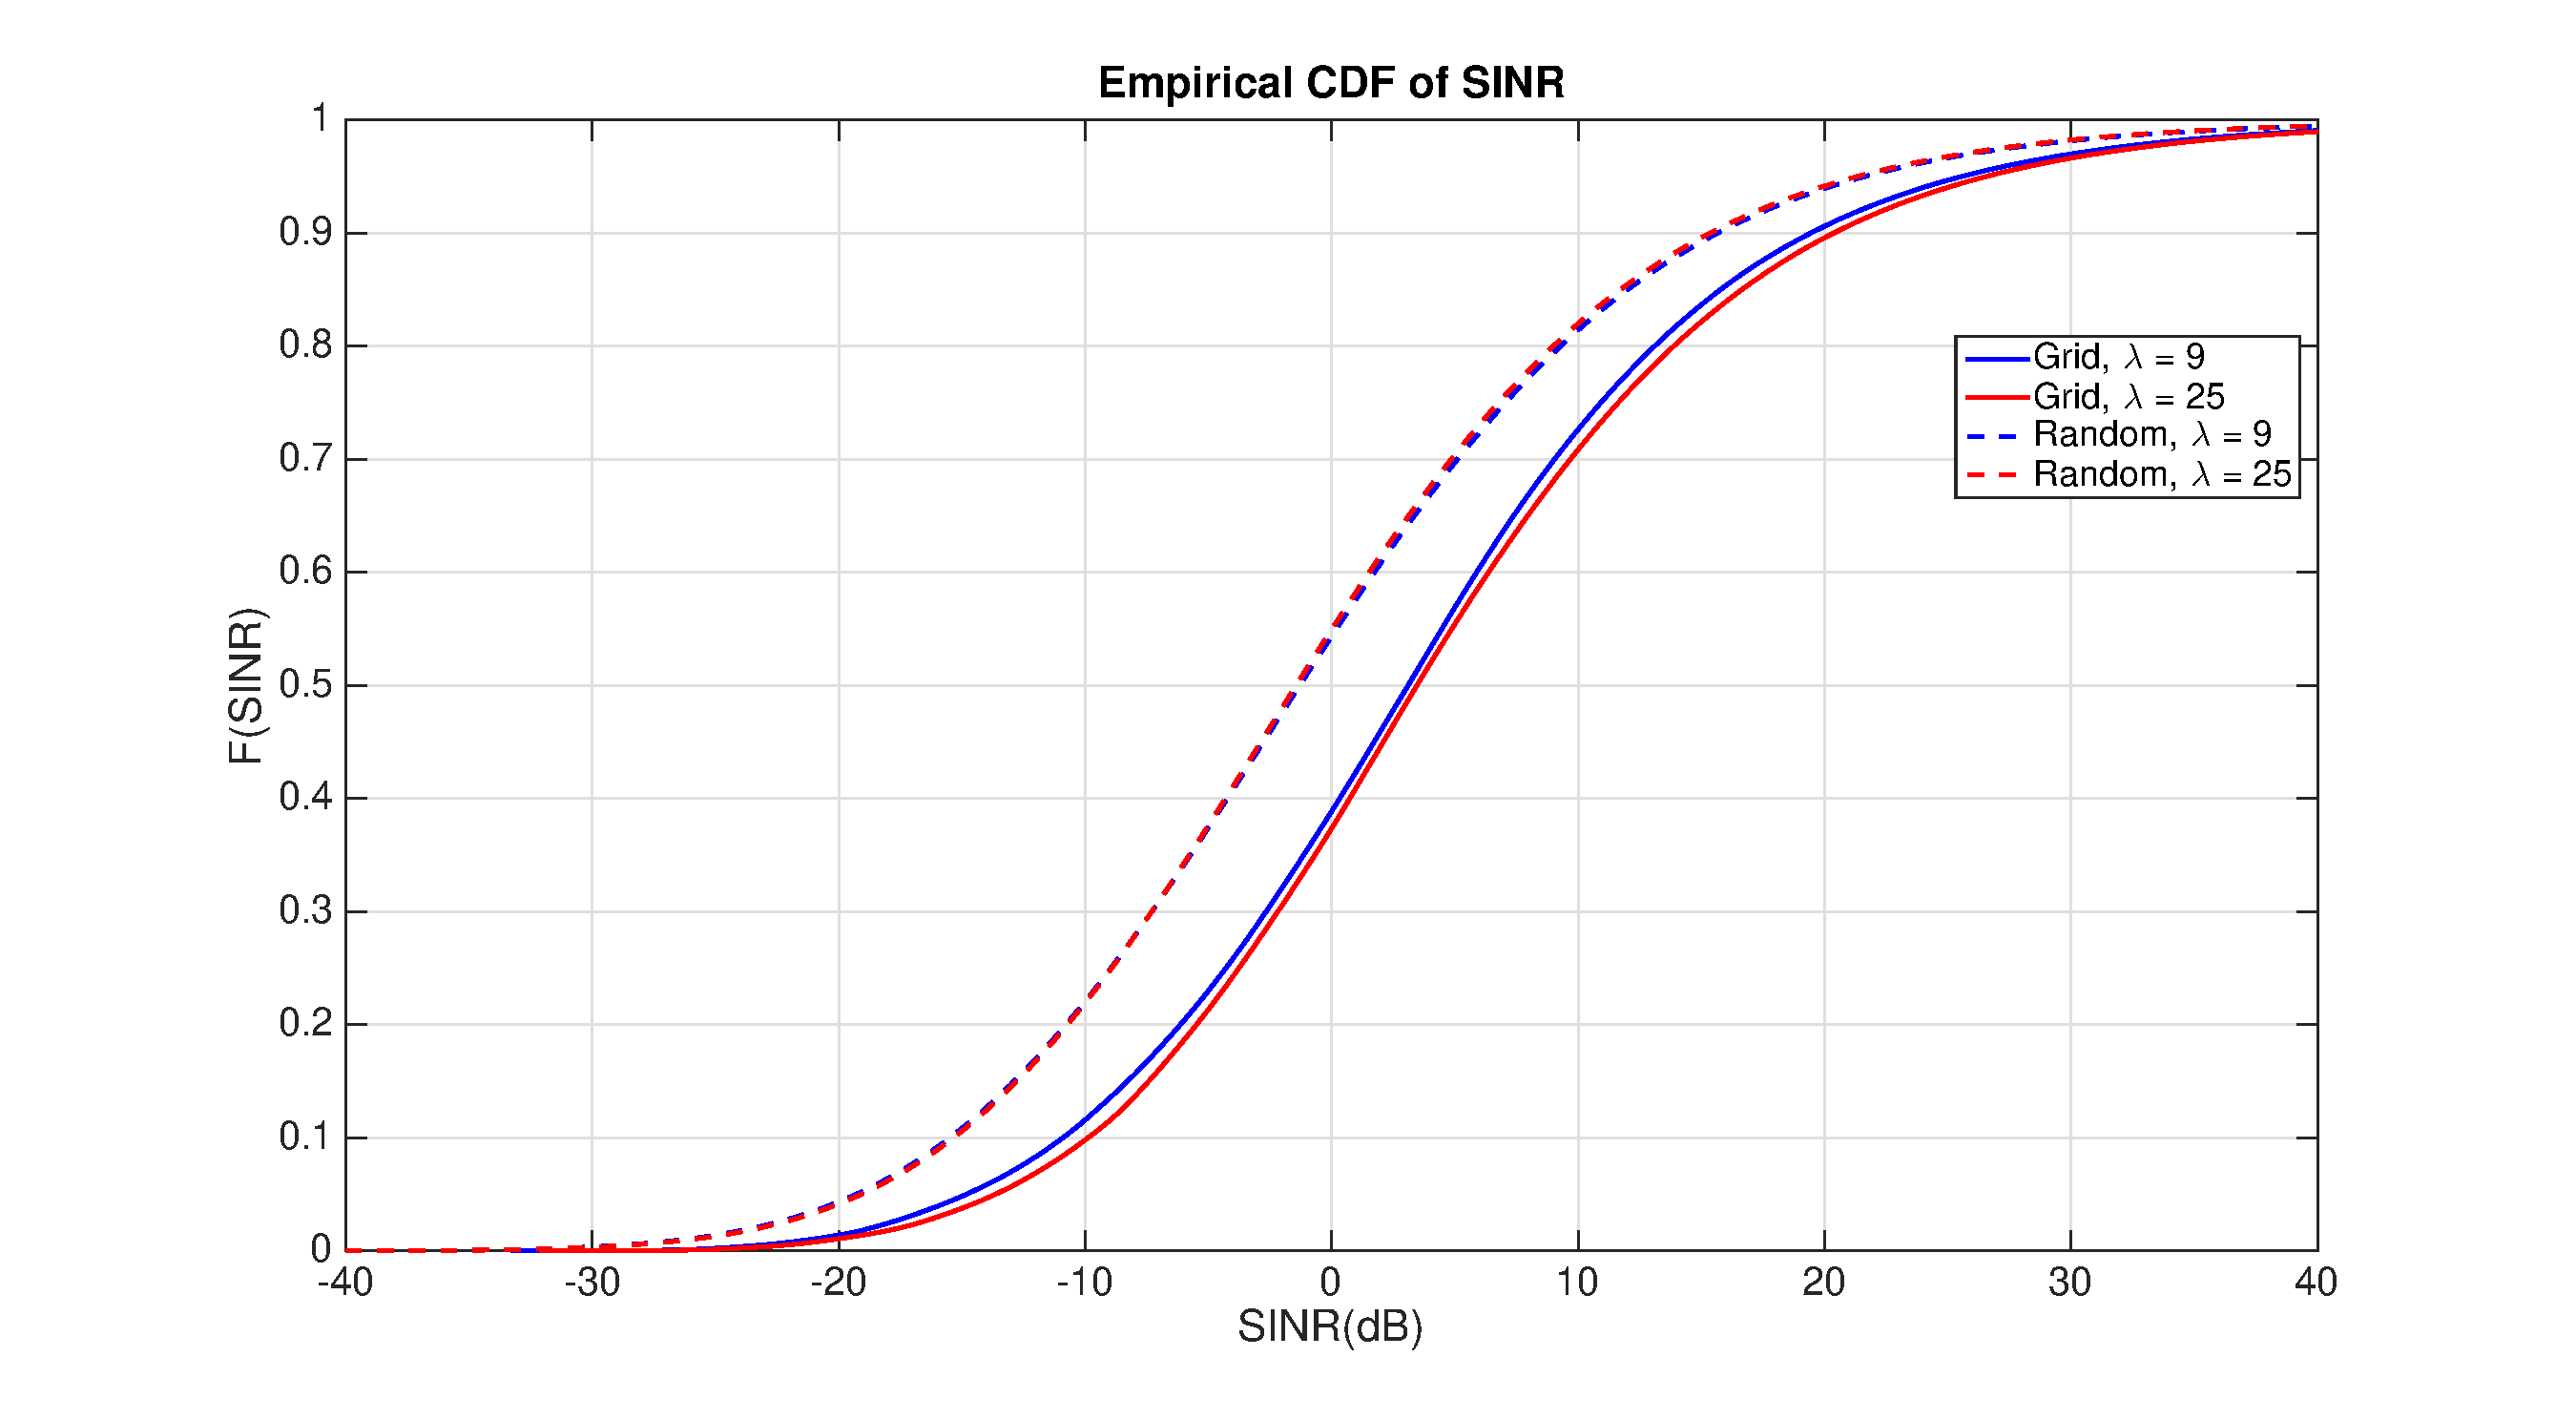
\includegraphics[width=8cm]{GridVSRandom.eps}
 \caption{CDF of SINR given Grid model and Random model (de-correlation distance: $20m$)}
 \label{4:cdf1}
 \end{figure}
 \begin{figure}
 \centering
 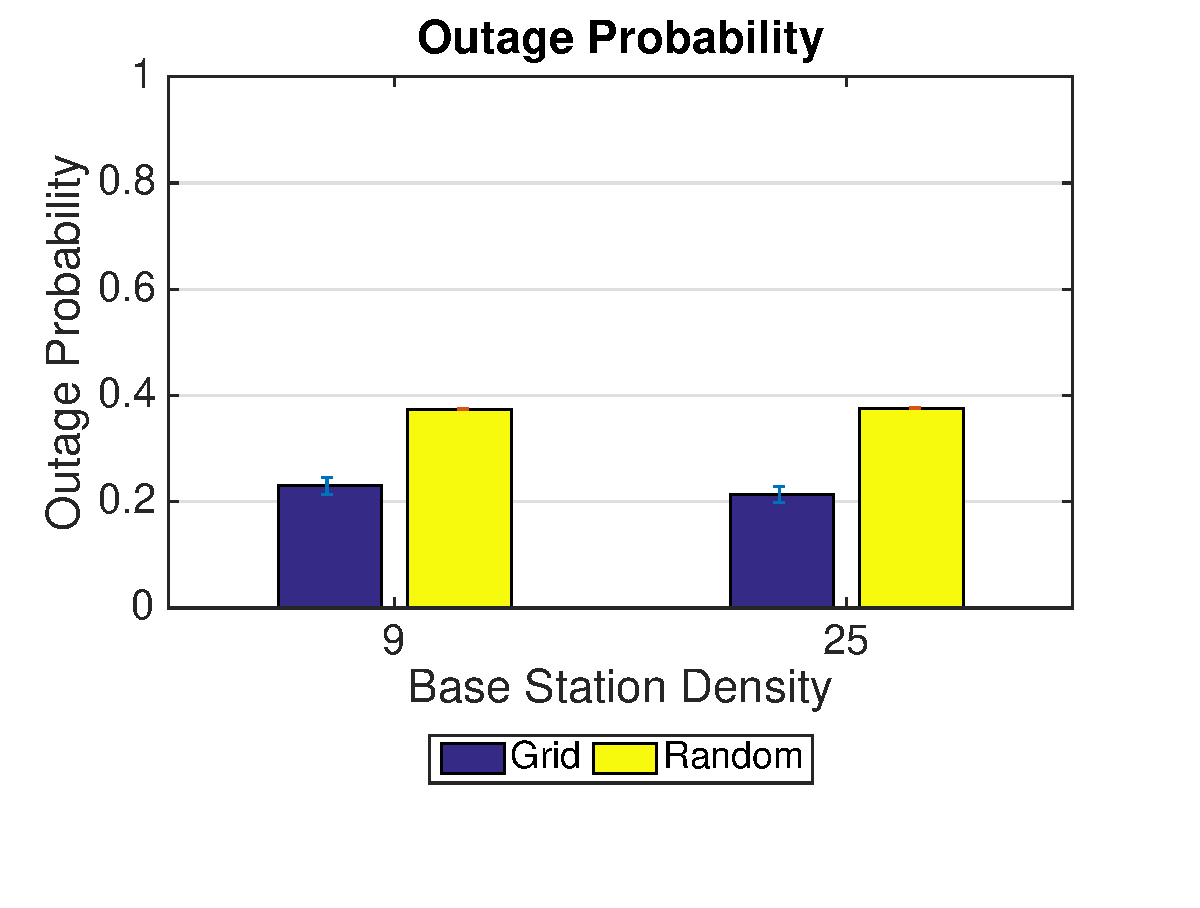
\includegraphics[width=8cm]{OutageProbGridVSRandom.eps}
 \caption{Outage probability given Grid model and Random model with $\gamma = -5dB$ (de-correlation distance: $20m$)}
 \label{4:outage1}
 \end{figure}


 \begin{figure*}
 \centering
 \subfigure[Independent shadow fading]{
 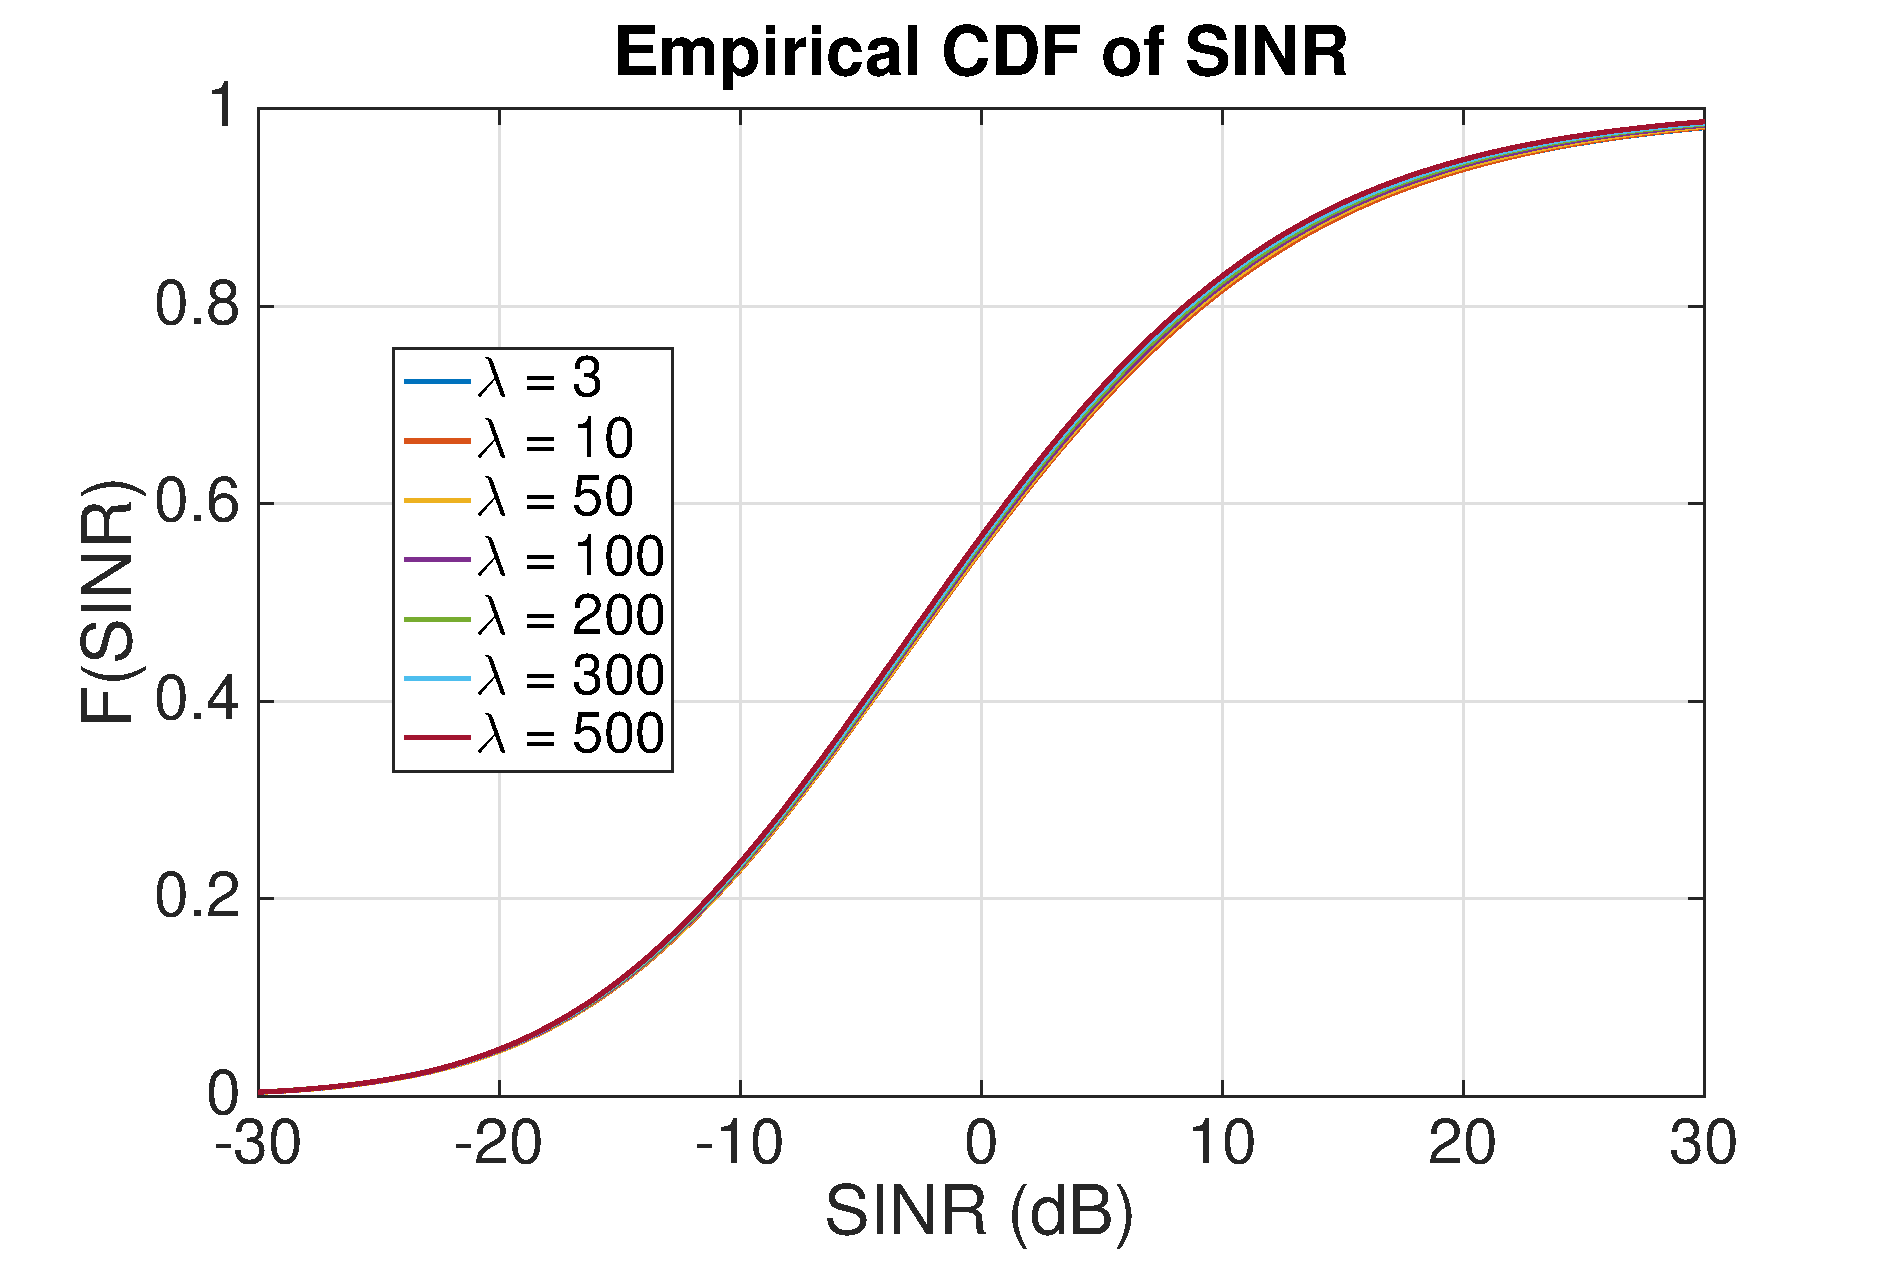
\includegraphics[width=5.5cm]{NBMax1000OutageProbCDFiid.eps}
 %\caption{CDF of SINR (the MS is connecting to the nearest BS, independent shadow fading}
 \label{4:Mode1}
 }
\hfil
\subfigure[Correlated shadow fading with $20m$ de-correlation distance]{
 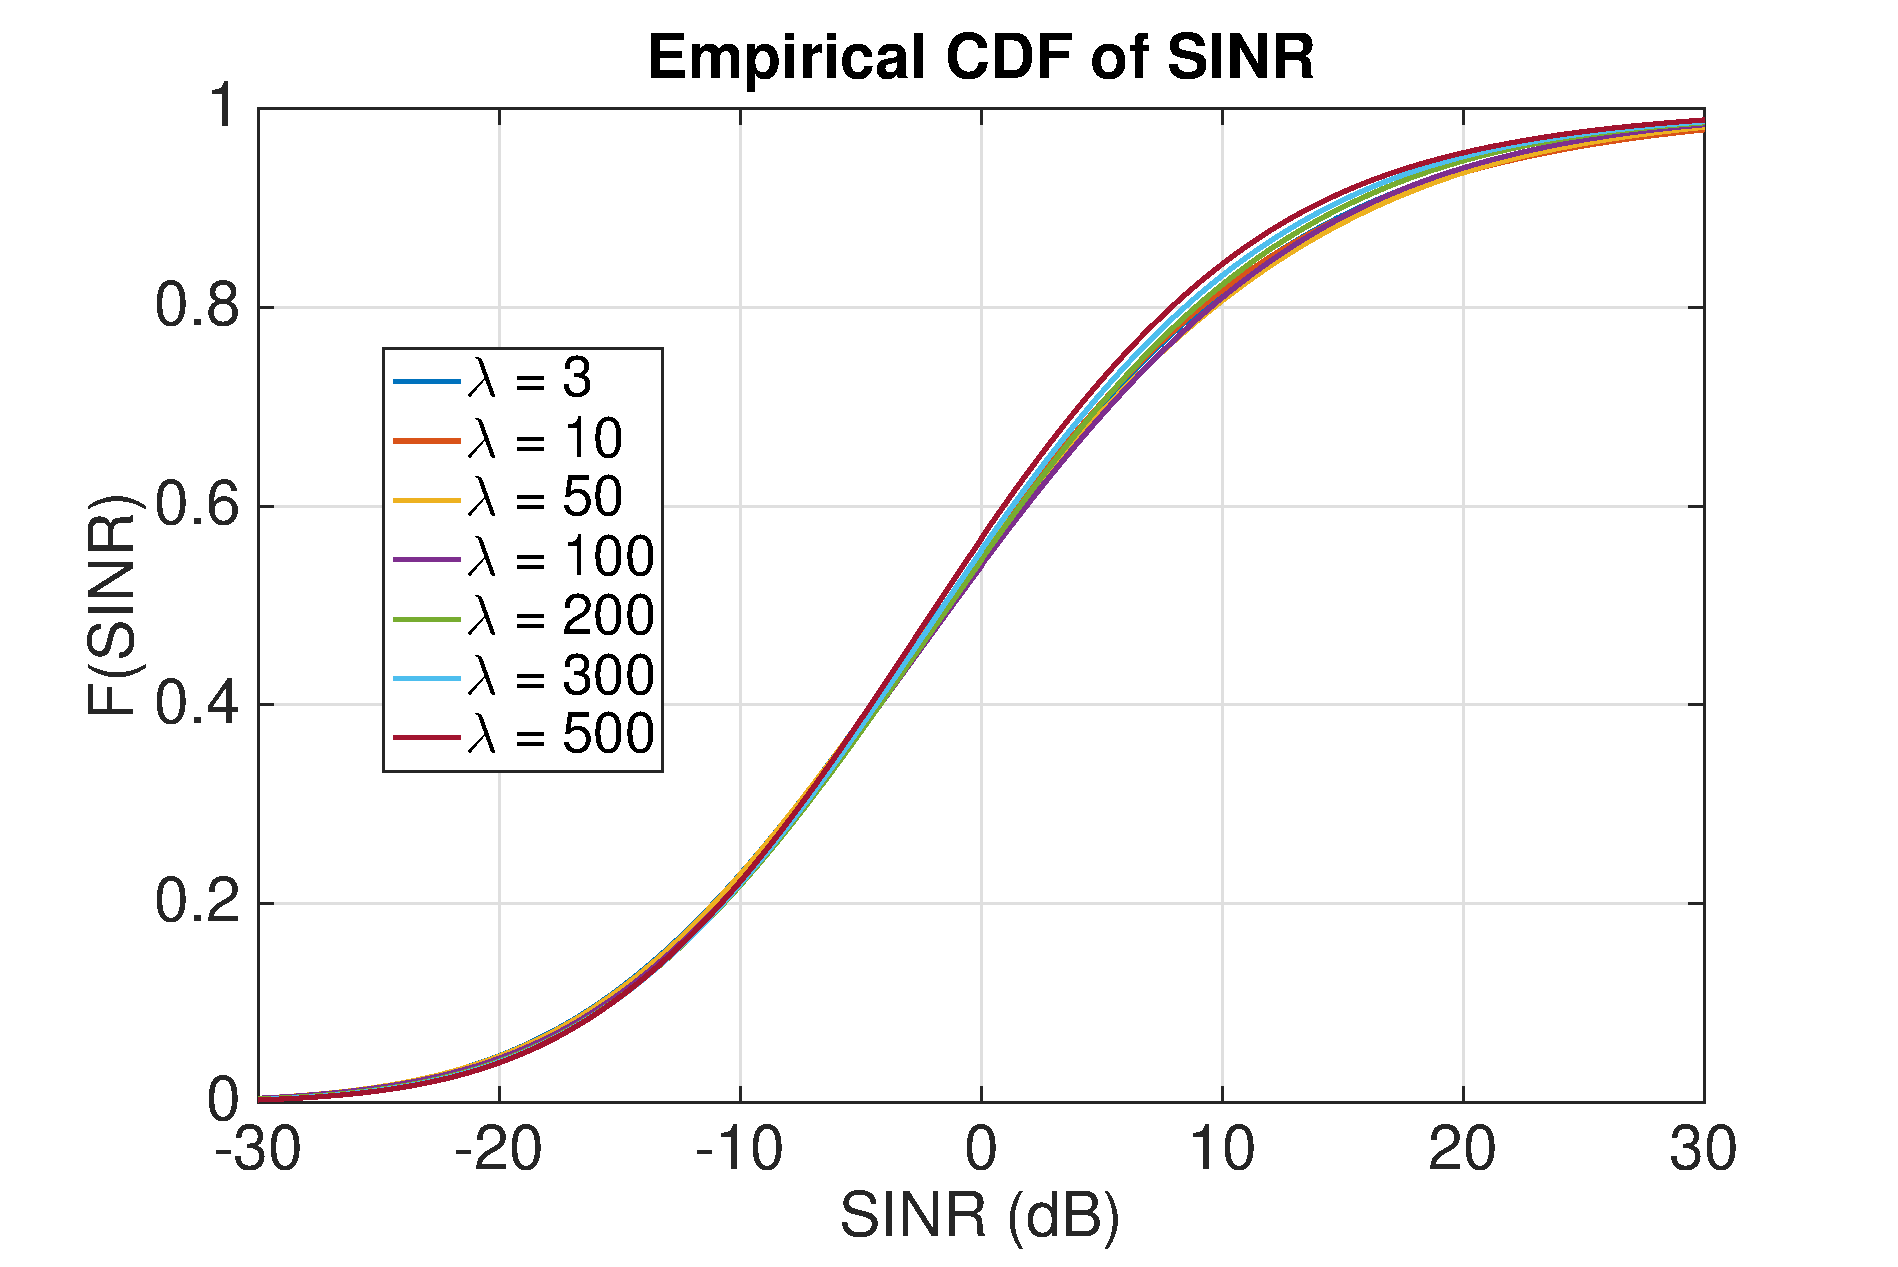
\includegraphics[width=5.5cm]{NBMax1000OutageProbCDFDeCorr20.eps}
 %\caption{CDF of SINR (the MS is connecting to the nearest BS, correlated shadow fading with 20m de-correlation distance}
 \label{4:Mode2}
 }
\hfil
\subfigure[Correlated shadow fading with $200m$ de-correlation distance]{
 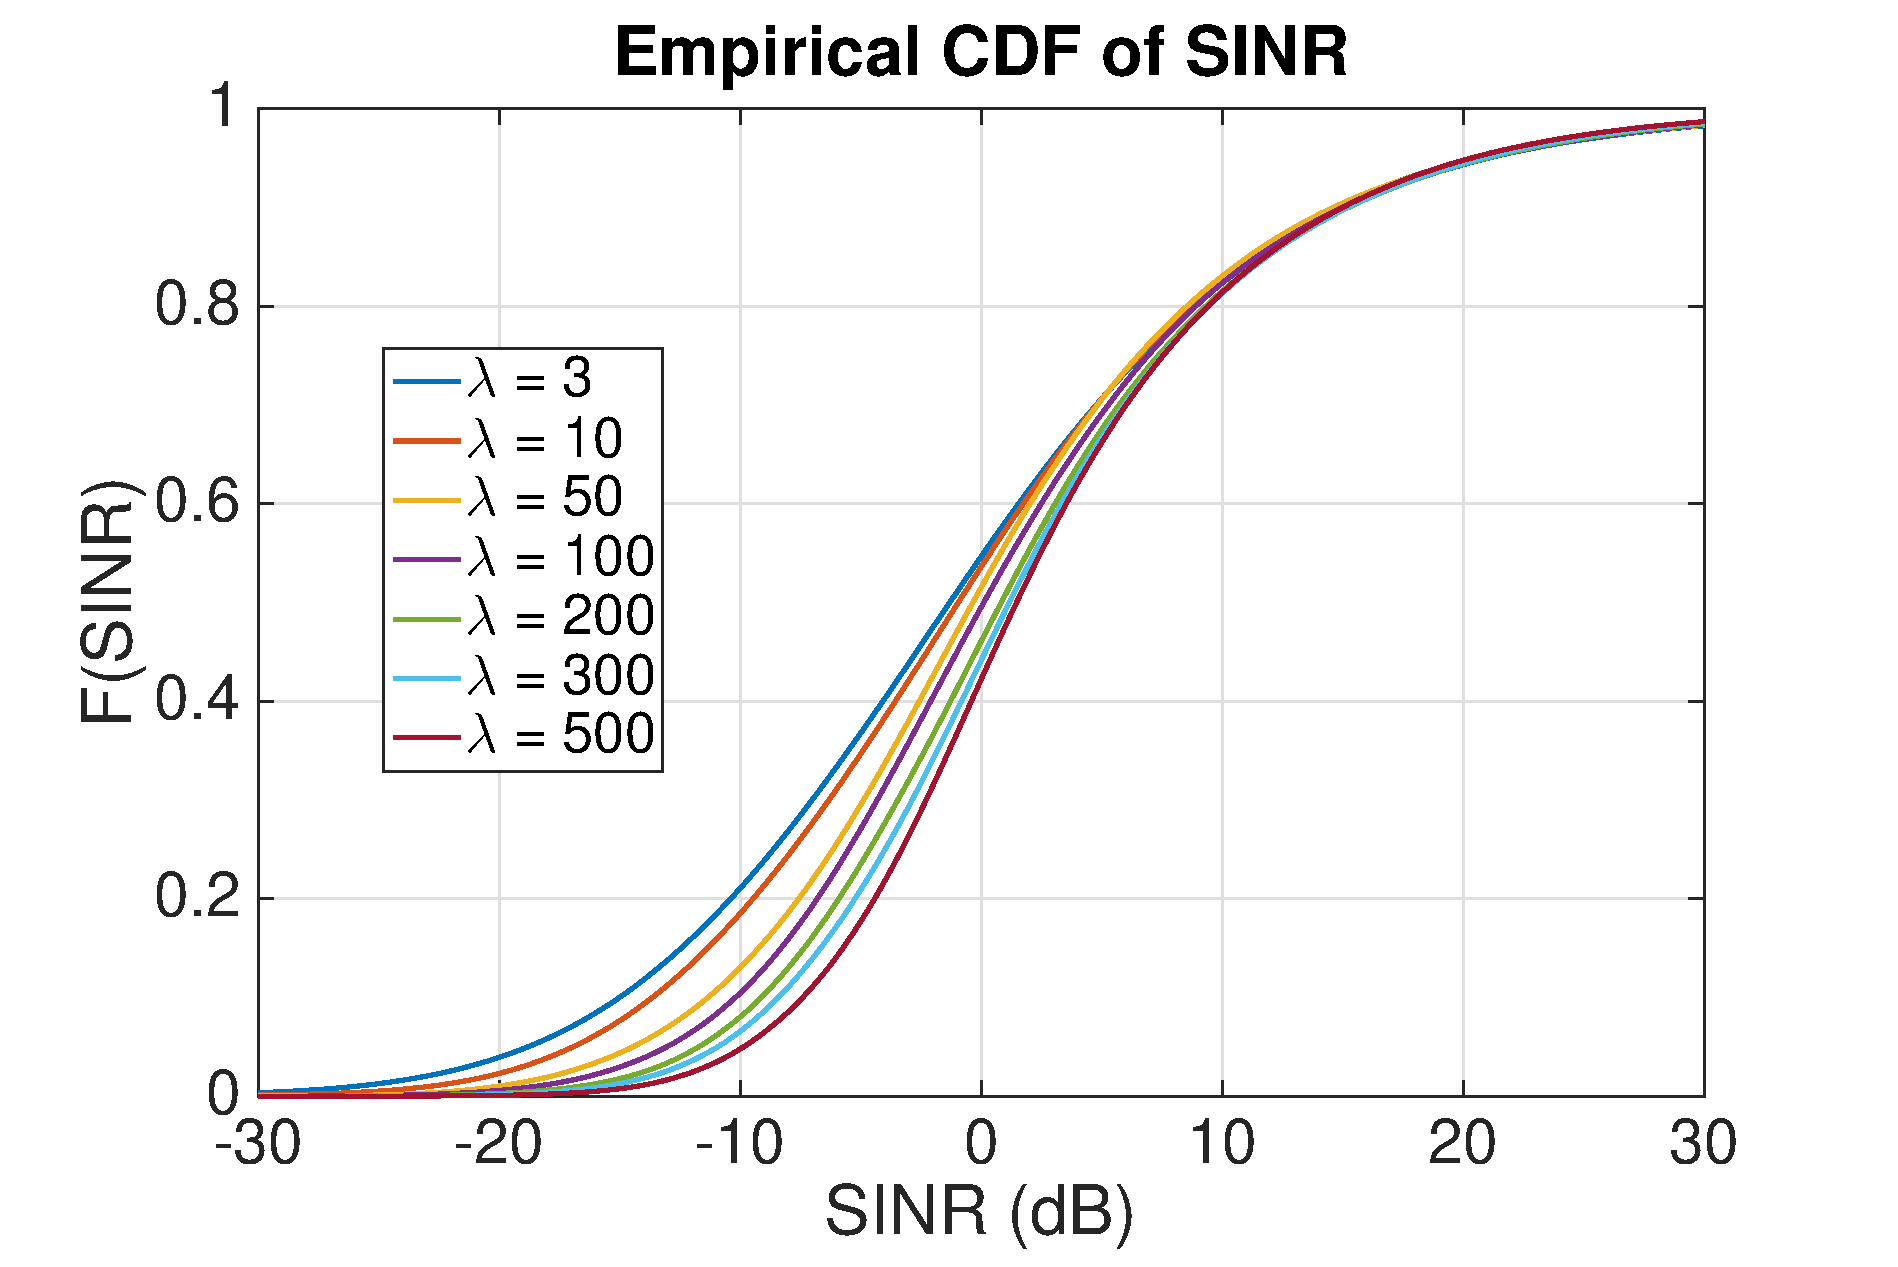
\includegraphics[width=5.5cm]{NBMax1000OutageProbCDFDeCorr200.eps}
 %\caption{CDF of SINR (the MS is connecting to the nearest BS, correlated shadow fading with 200m de-correlation distance}
 \label{4:Mode3}
 }
 \caption{CDF of MS's receiving SINR when connecting to the Nearest BS (three different shadow fading modes and different BS densities).}
\label{nearestBS}
 \end{figure*}


 \begin{figure*}
 \centering
 \subfigure[Independent shadow fading]{
 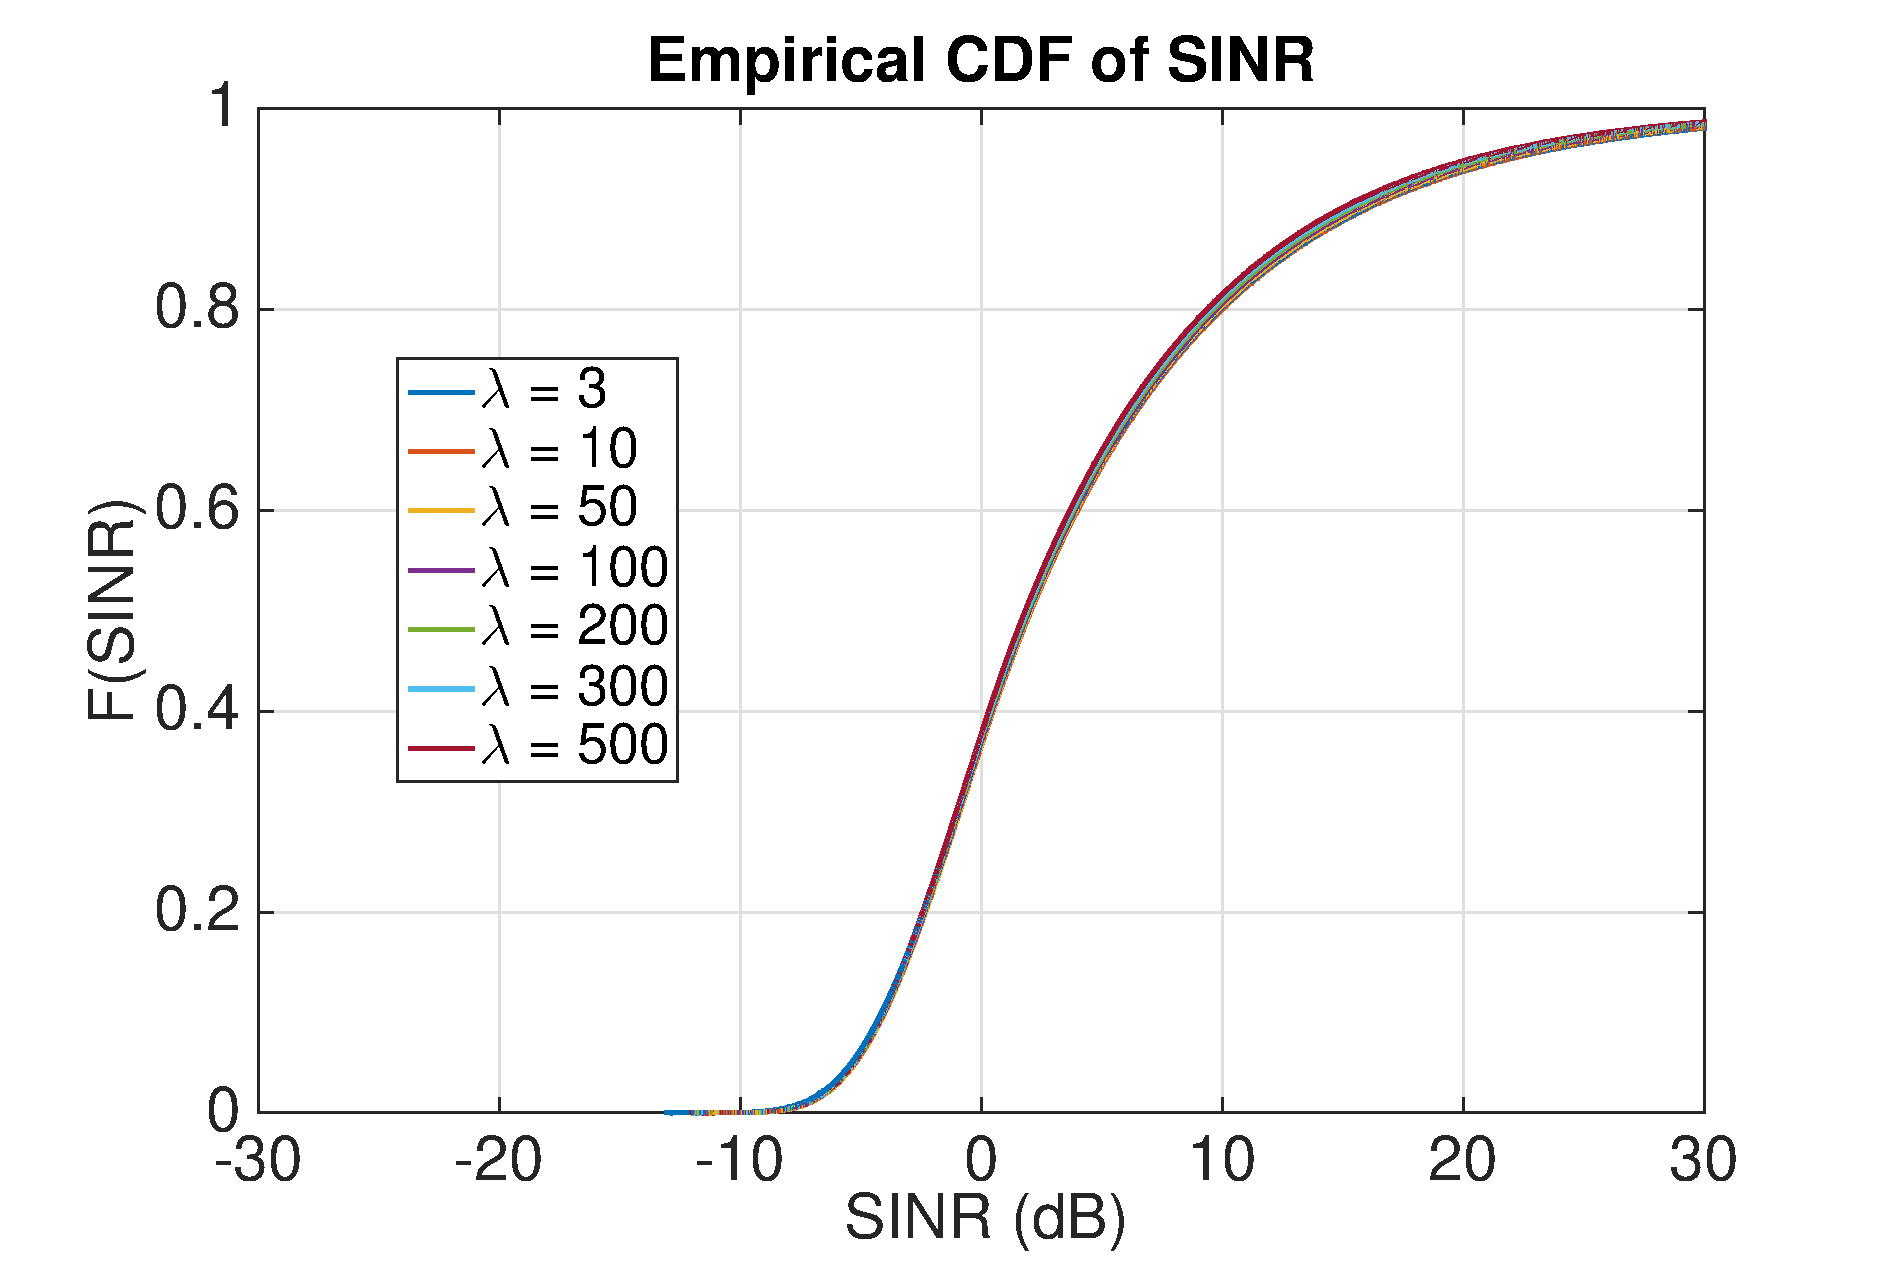
\includegraphics[width=5.5cm]{MaxMax1000OutageProbCDFiid.eps}
% \caption{CDF of SINR (the MS is connecting to the strongest BS, independent shadow fading}
 \label{4:Mode12}}
 \hfil
\subfigure[Correlated shadow fading with $20m$ de-correlation distance]{
 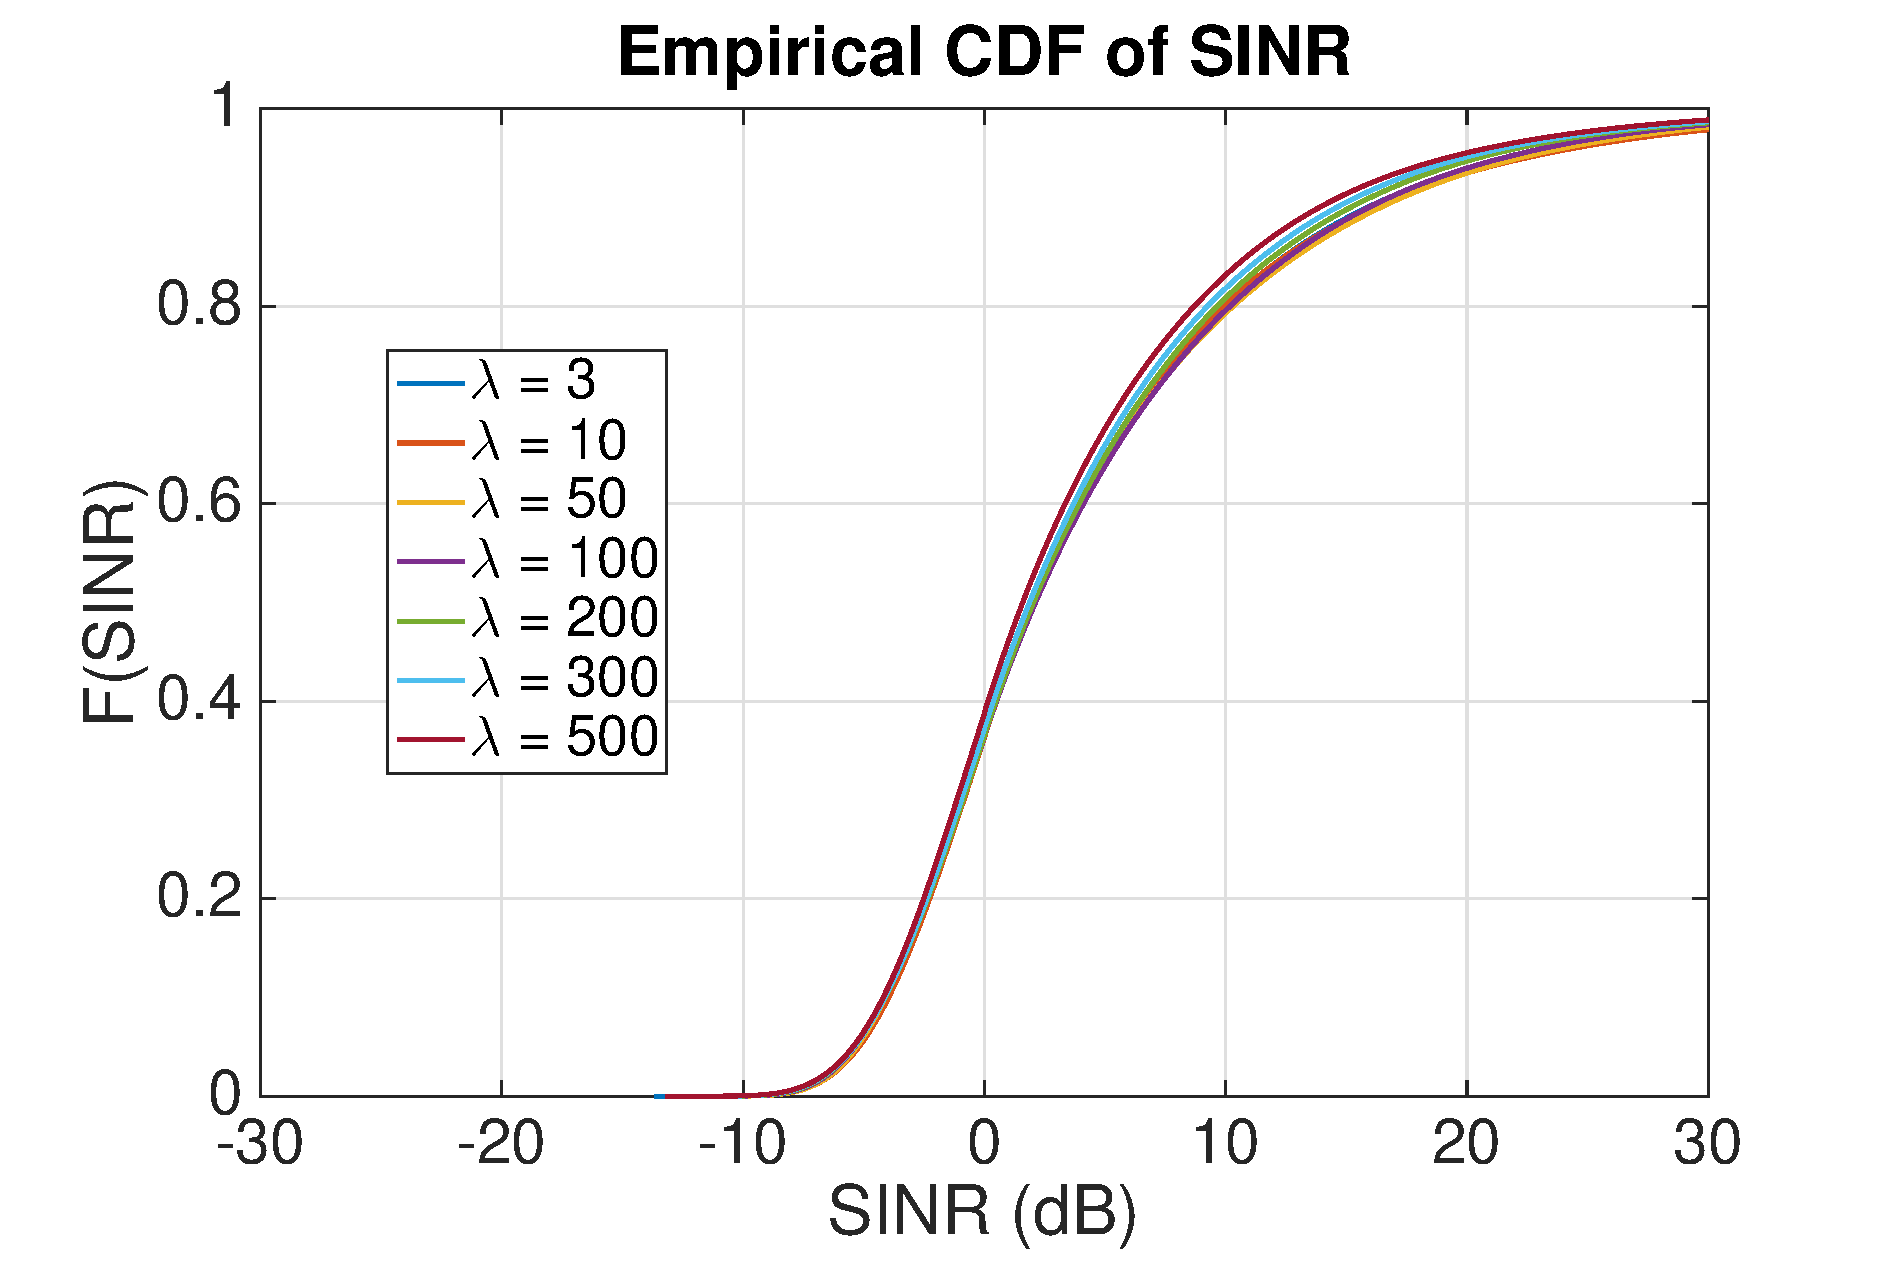
\includegraphics[width=5.5cm]{MaxMax1000OutageProbCDFDeCorr20.eps}
 %\caption{CDF of SINR (the MS is connecting to the strongest BS, correlated shadow fading with 20m de-correlation distance}
 \label{4:Mode22}
 }
\hfil
\subfigure[Correlated shadow fading with $200m$ de-correlation distance]{
 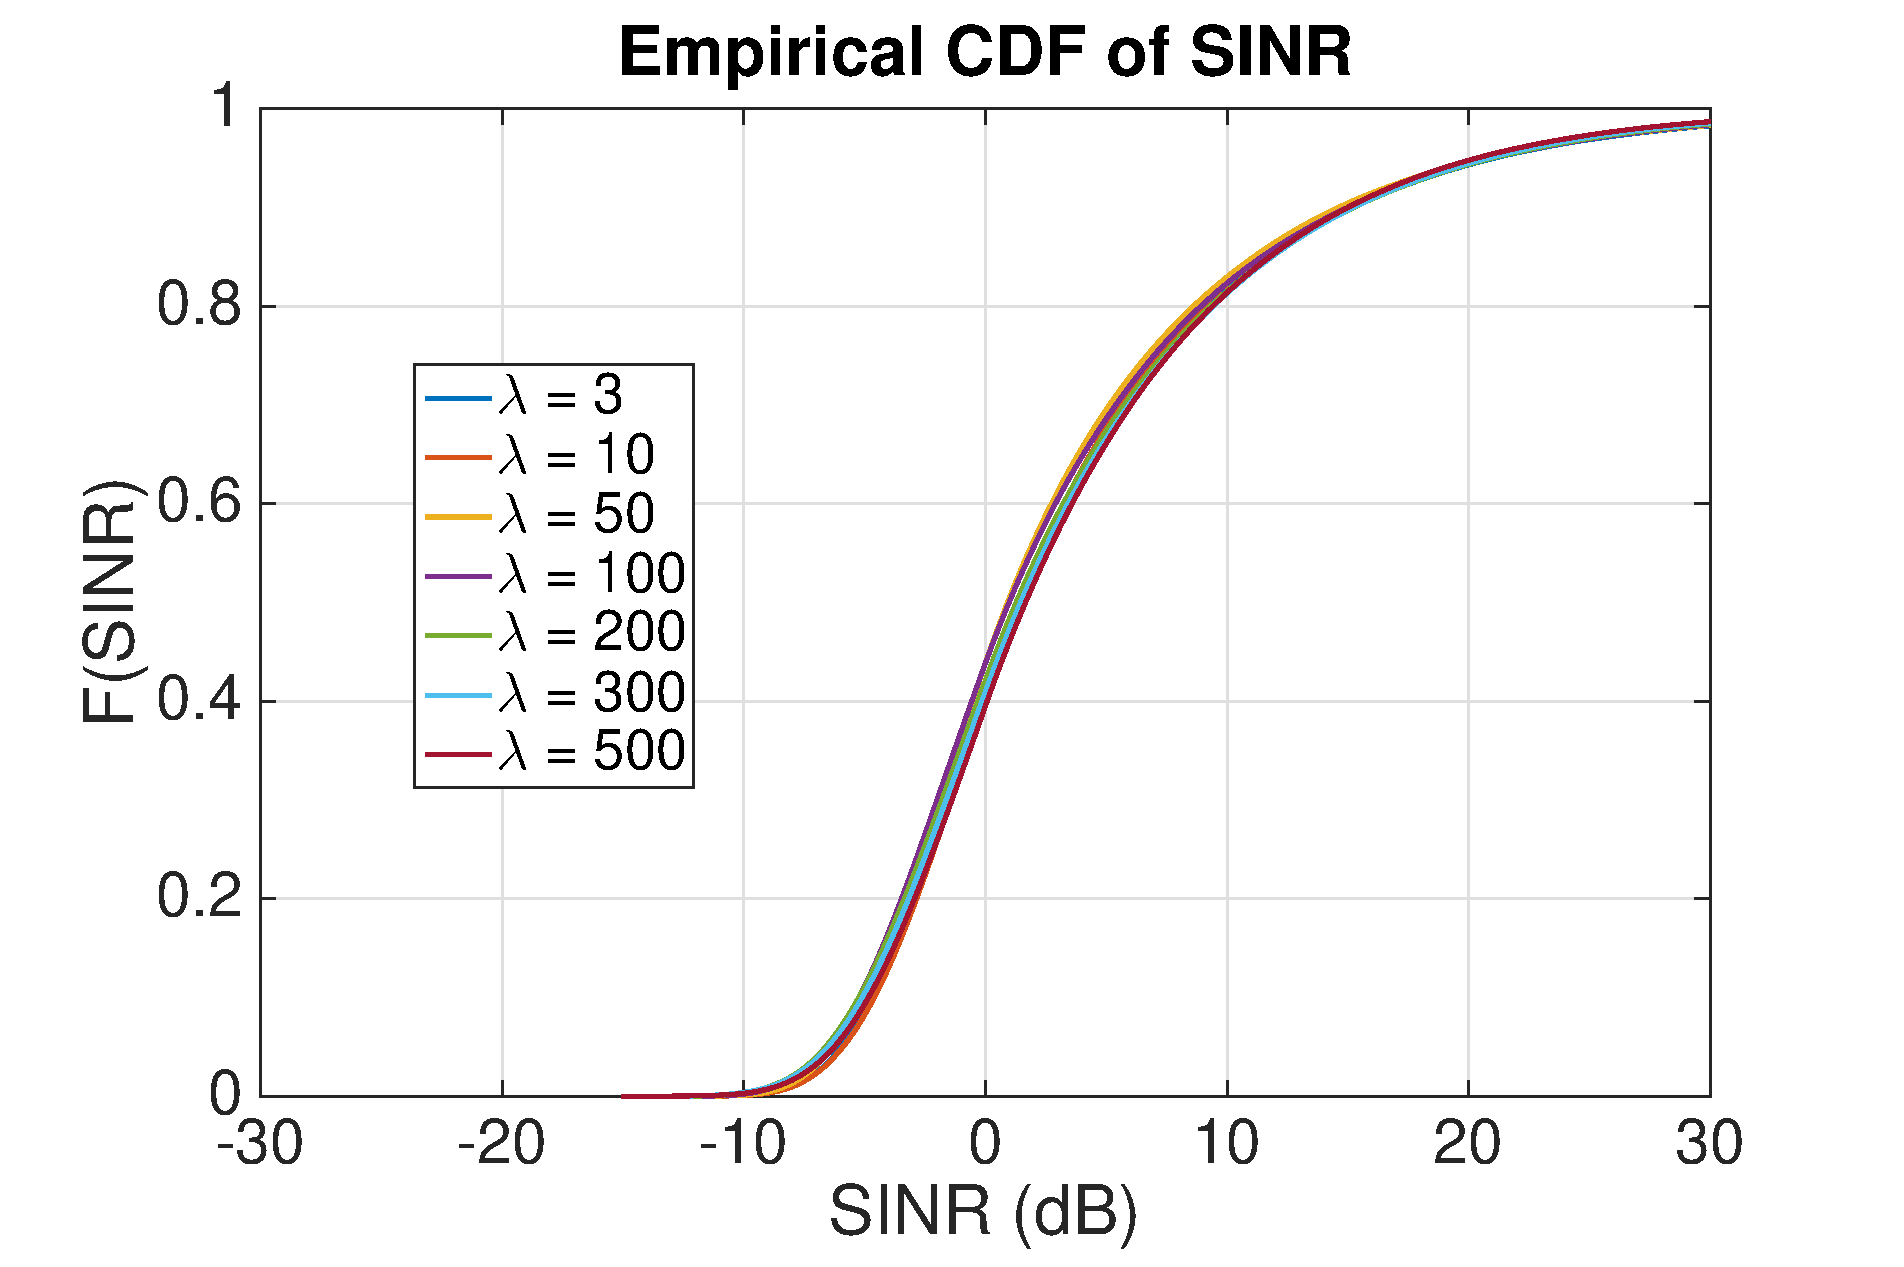
\includegraphics[width=5.5cm]{MaxMax1000OutageProbCDFDeCorr200.eps}
% \caption{CDF of SINR (the MS is connecting to the strongest BS, correlated shadow fading with 200m de-correlation distance}
 \label{4:Mode32}
 }
 \caption{CDF of MS's receiving SINR when connecting to the Strongest BS (three different shadow fading modes and different BS densities).}
\label{strongestBS}
 \end{figure*}

 \par For the Random model, the SINR distribution and the outage probability of different BS densities are investigated for both the Nearest BS mode and the Strongest BS mode. Simulations are implemented under independent shadow fading and correlated shadow fading. CDF curves of SINR are generated and the outage probability given the SINR threshold being $-5dB$ are presented for increasing BS densities. Fig. \ref{nearestBS} shows the SINR of the MS when connecting to the nearest BS. From Fig. \ref{4:Mode1} and Fig. \ref{4:Mode2}, it is obvious that the CDF curves are overlapping each other, which means increasing BS density does not change the CDF of SINR. From this we can conclude, under the circumstance that the shadow fading is independent or the de-correlation distance of the correlated shadow fading is small, increasing the BS density will not improve the system performance in terms of reducing the outage probability. Fig. \ref{4:Mode3}  illustrates that CDF of SINR improves (curve moves toward the bottom-right corner) as we increase the BS density. Therefore, increasing the BS density will result in better system performance when the de-correlation distance is large, by reducing the outage probability. Fig. \ref{fig: outprob1} shows the outage probability of different correlated shadow fading models and different BS densities when SINR threshold is set to $-5dB$. These blue and green bars suggest that increasing the BS density will not decrease the outage probability when shadow fading is independent or correlated with $20m$ de-correlation distance. Meanwhile, these yellow bars suggest that when the de-correlation distance is $200m$, increasing the BS density will reduce the outage probability. For example, when the BS density is $3$, the outage probability is around $38\%$. Increasing the BS density to $500$, the outage probability decreases to $18\%$. The above simulation results suggest that when the de-correlation distance is relatively large, and the MS is connecting to the nearest BS, increasing the BS density will reduce the outage probability and improve the system performance.



 \begin{figure}
 \centering
 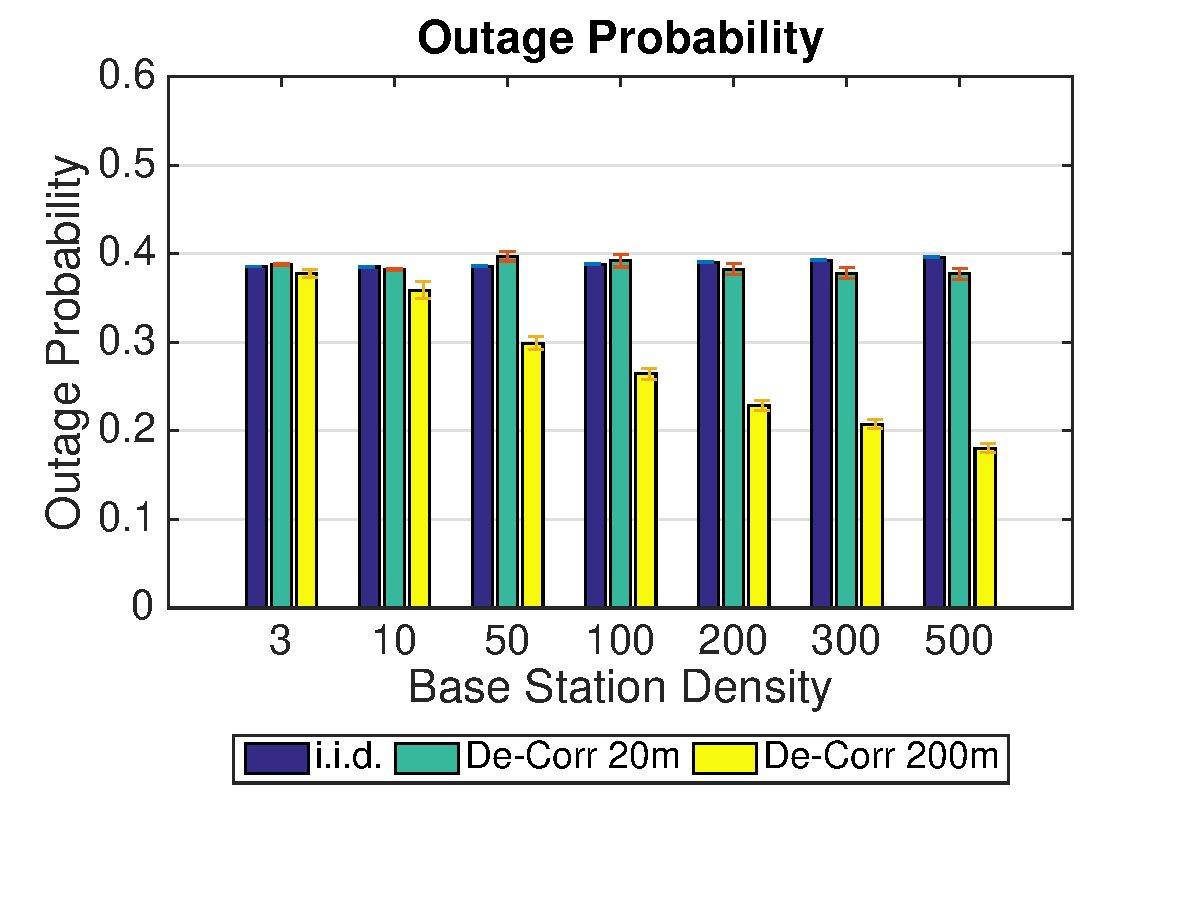
\includegraphics[width=9cm]{NBMax1000OutageProbThresh-5iid.eps}
 \caption{Outage probability given $-5dB$ SINR threshold}
 \label{fig: outprob1}
 \end{figure}
 \begin{figure}
 \centering
 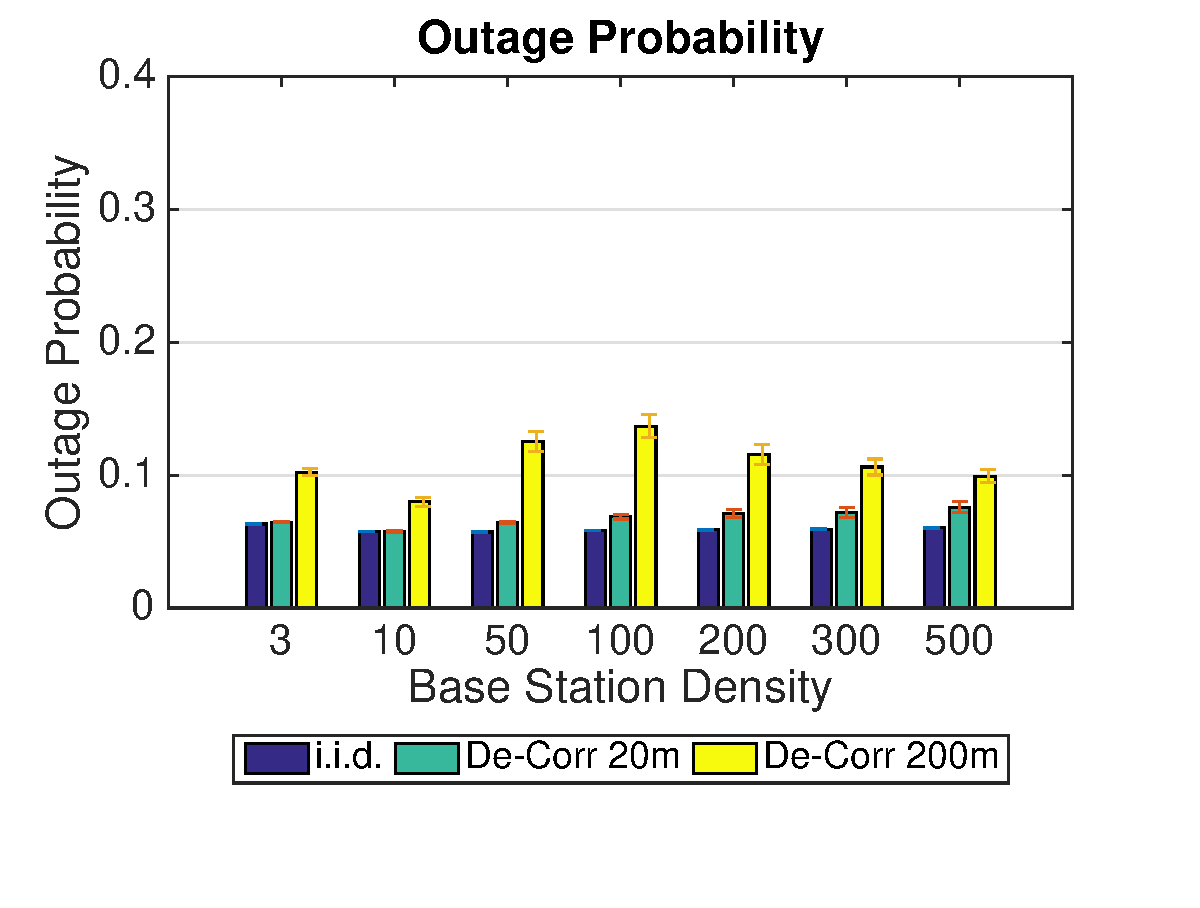
\includegraphics[width=9cm]{MaxMax1000OutageProbThresh-5iid.eps}
 \caption{Outage probability given $-5dB$ SINR threshold}
 \label{fig: outprobs2}
 \end{figure}
 \begin{figure*}
 \centering
 \subfigure[Independent shadow fading]{
 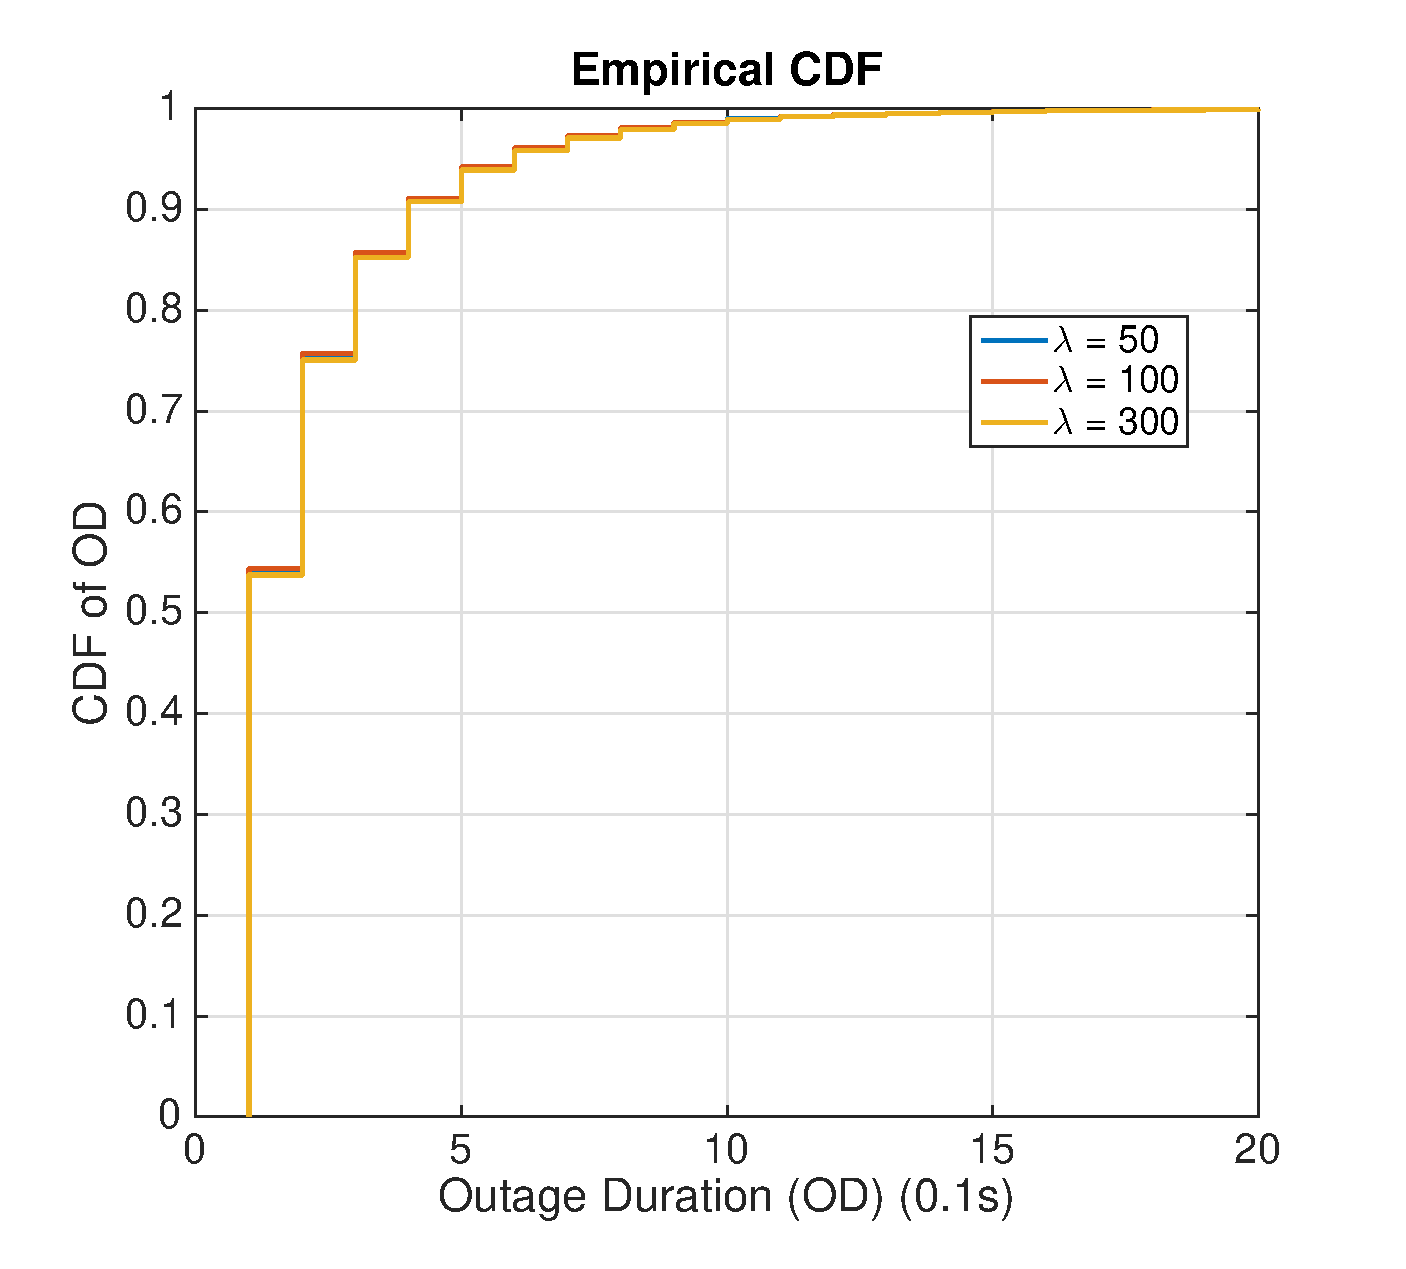
\includegraphics[width=5.5cm]{ODthresh-5iidNB.eps}
 %\caption{CDF of Outage Durations when the MS is connecting to the Nearest BS with independent shadow fading}
 \label{iid1}
 }
 \hfil
  \subfigure[Correlated shadow fading with $20m$ de-correlation distance]{
 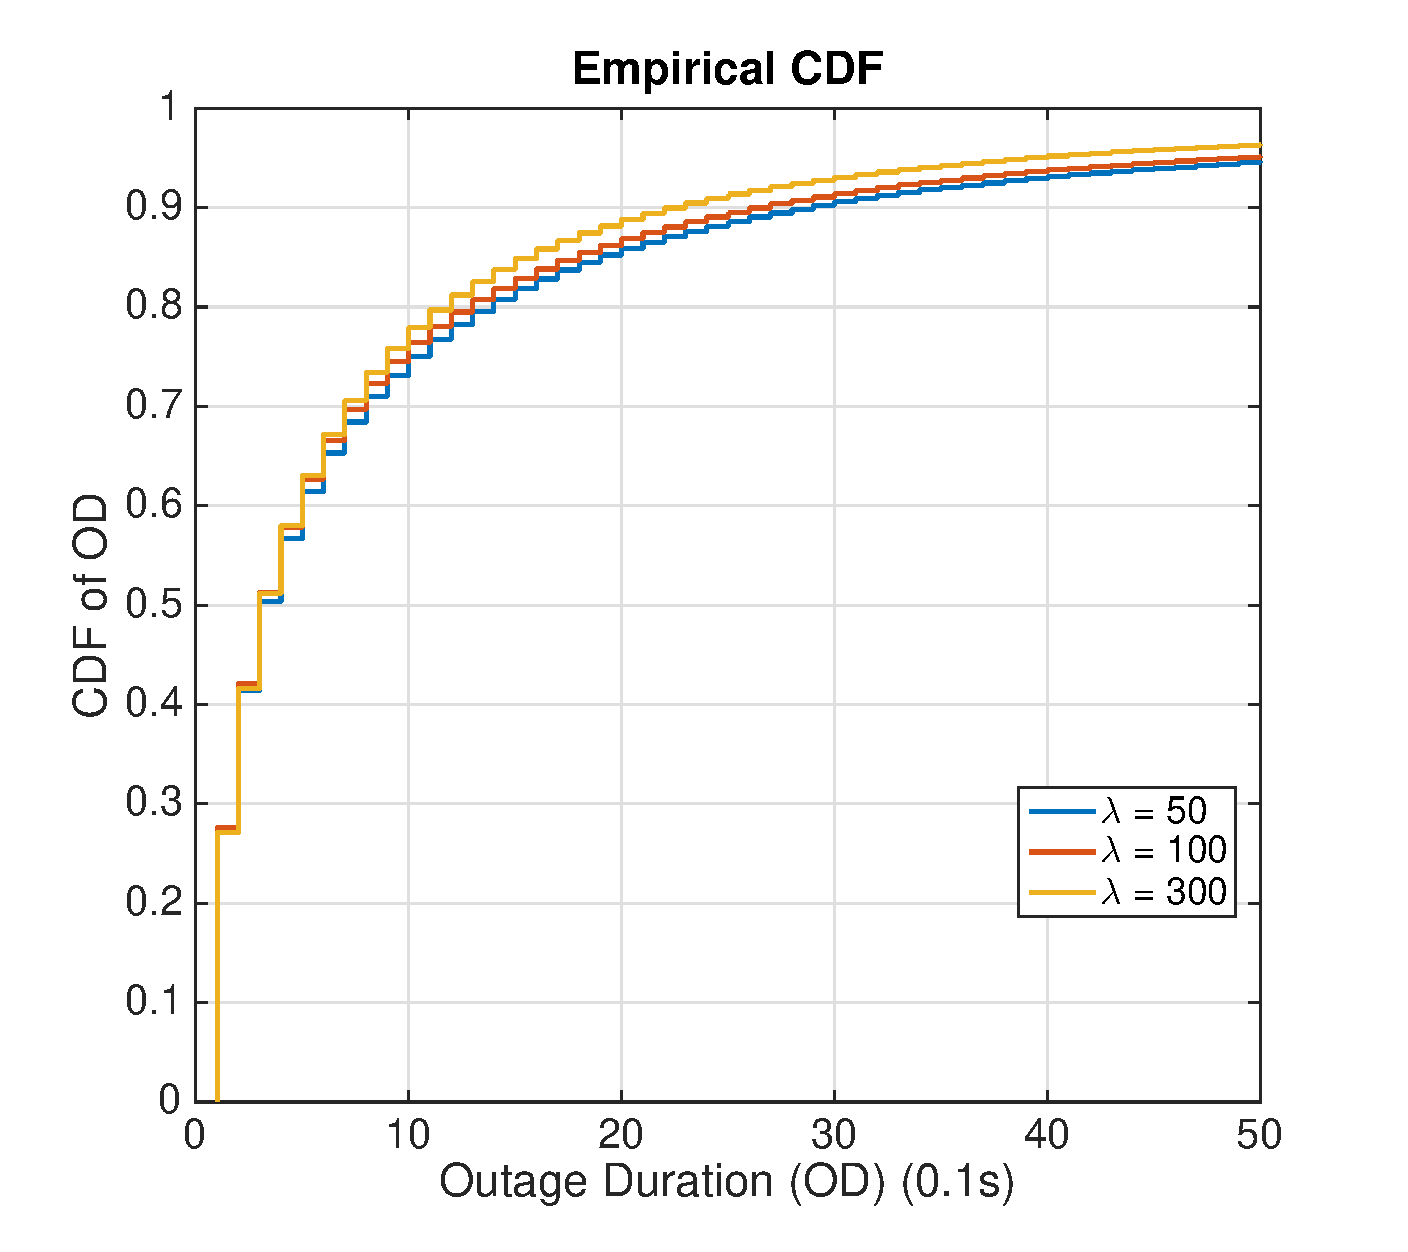
\includegraphics[width=5.5cm]{ODthresh-5DeCorr20NBMode2.eps}
% \caption{CDF of Outage Durations when MS is connecting to the Nearest BS with correlated shadowing (de-correlation distance: 200m)}
 \label{corr201}
 }
 \hfil
   \subfigure[Correlated shadow fading with $200m$ de-correlation distance]{
 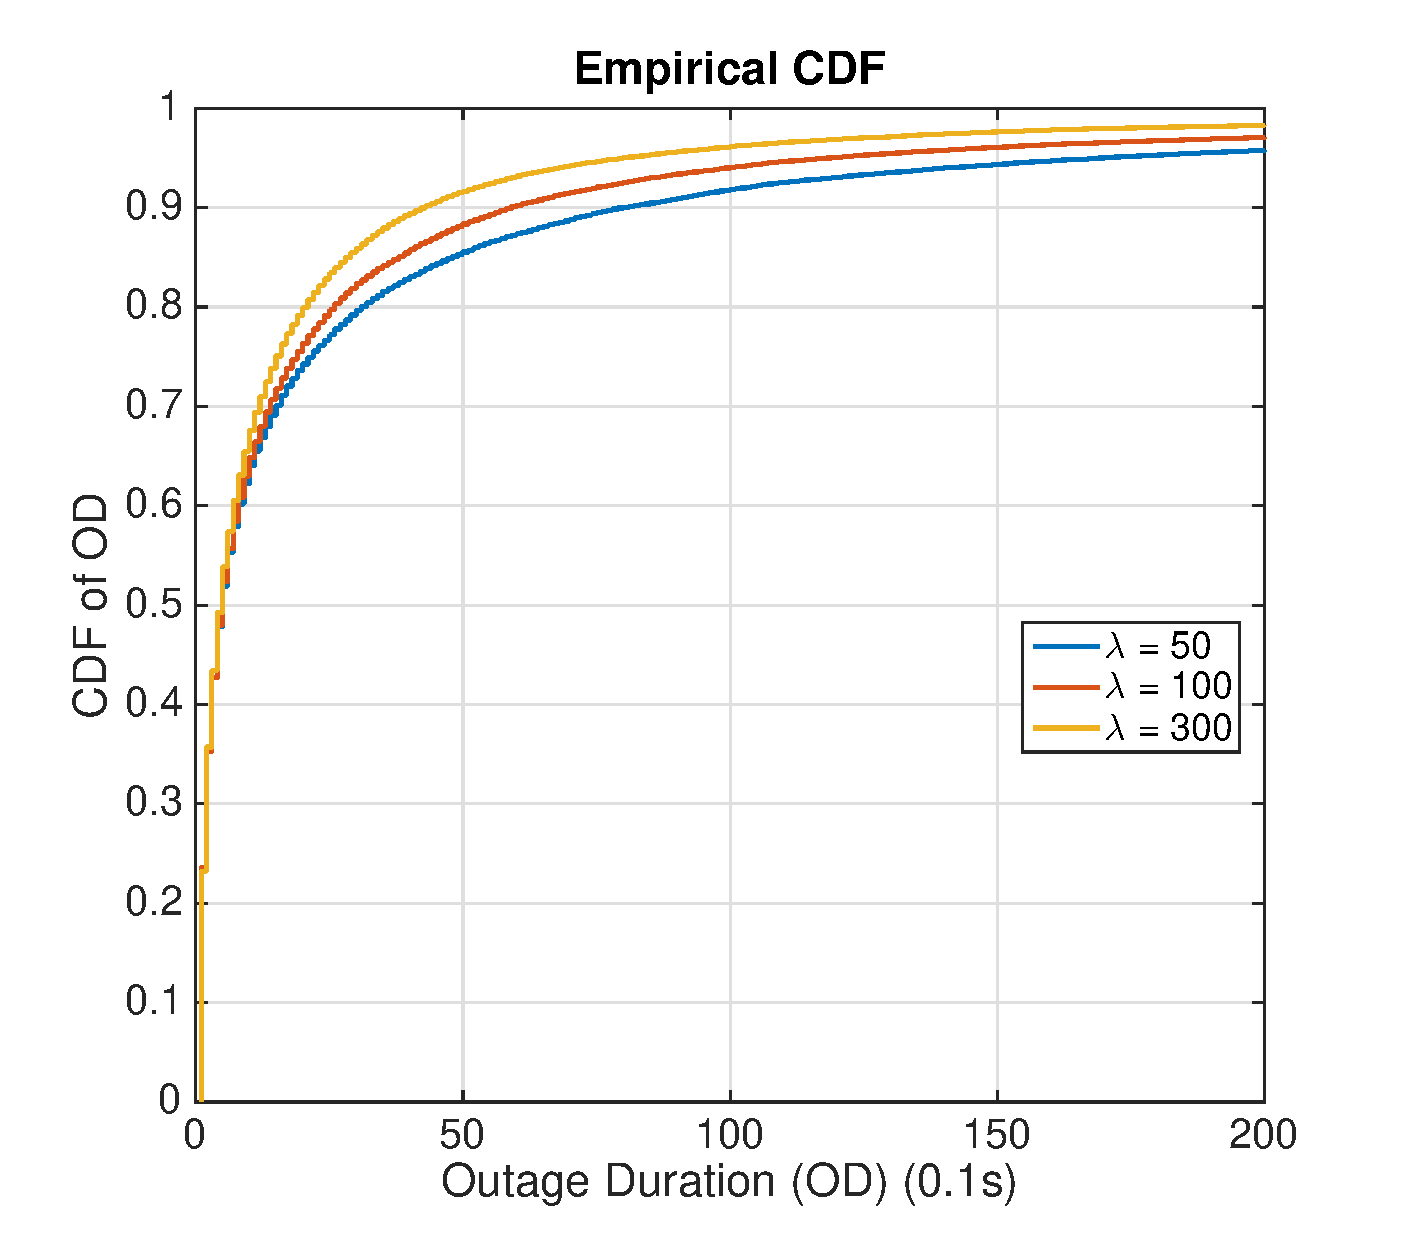
\includegraphics[width=5.5cm]{ODthresh-5DeCorr200NBMode2.eps}
% \caption{CDF of Outage Durations when MS is connecting to the Nearest BS with correlated shadowing (de-correlation distance: 200m)}
 \label{corr2001}
 }
 \caption{CDF of Outage Durations when MS is connecting to the Strongest BS with correlated shadowing}
 \label{outageduration0}
 \end{figure*}
 \begin{figure*}
 \centering
 \subfigure[Independent shadow fading]{
 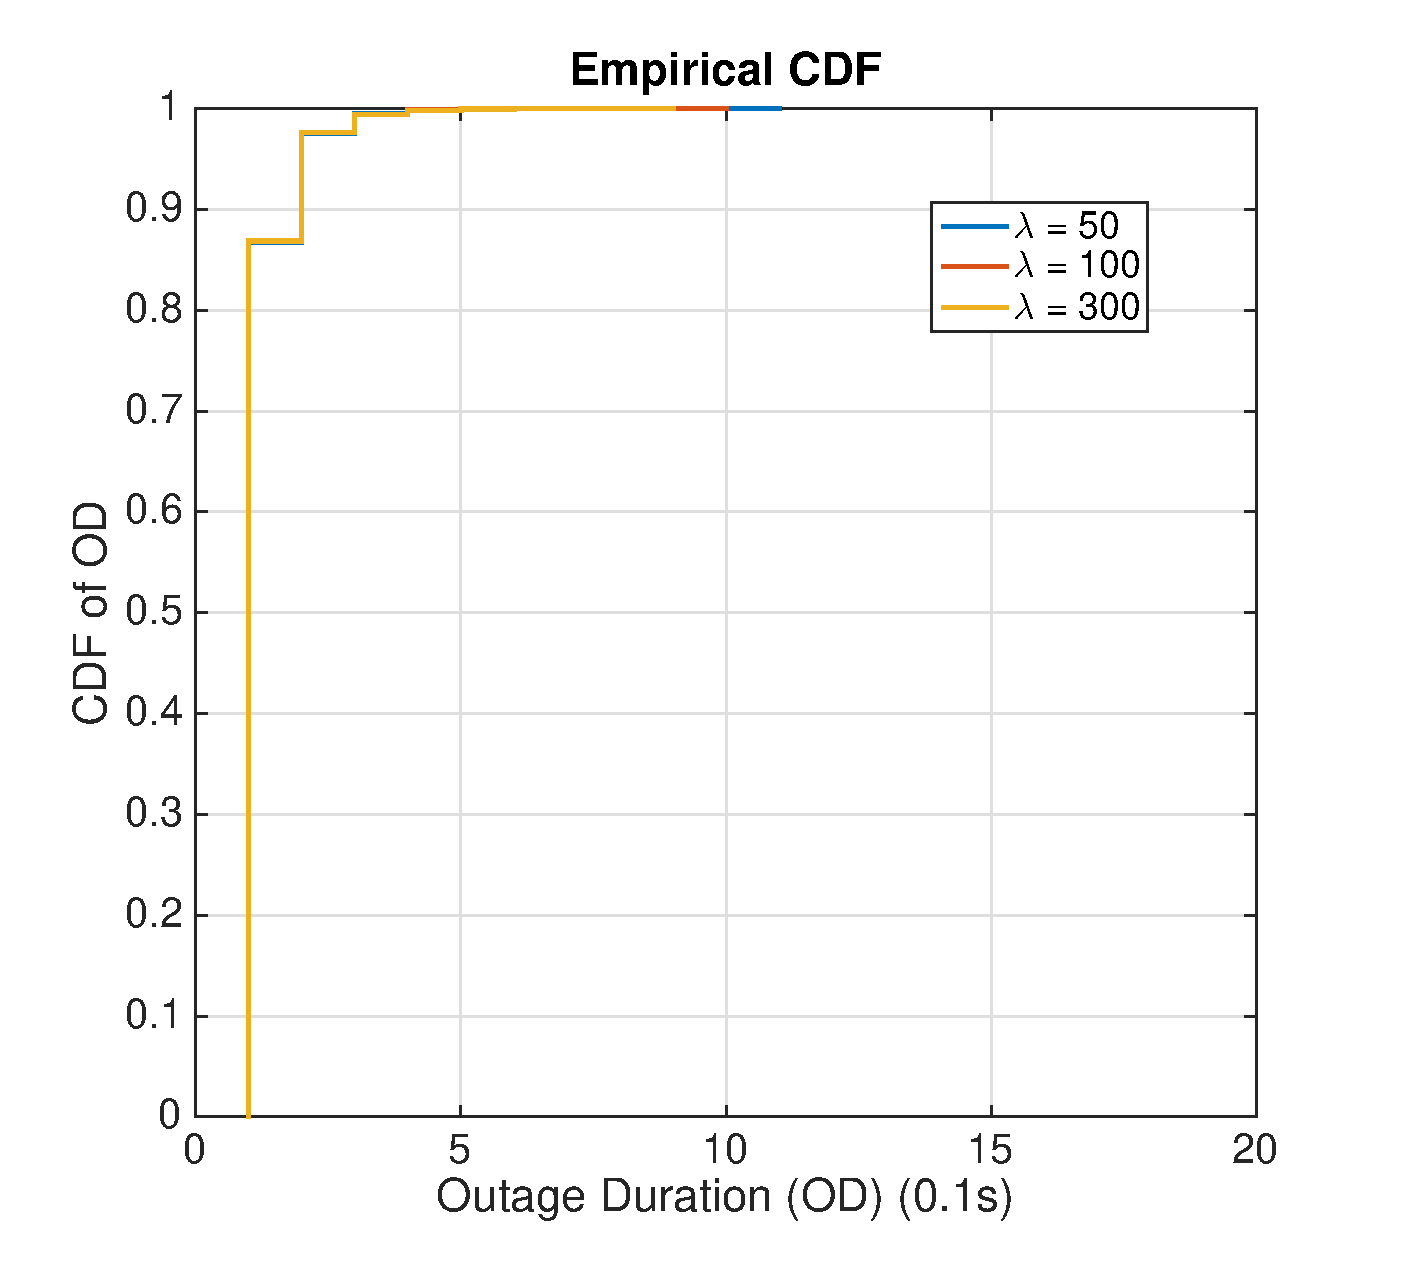
\includegraphics[width=5.5cm]{ODthresh-5iidMax.eps}
 %\caption{CDF of Outage Durations when the MS is connecting to the Strongest BS with independent shadow shadowing}
 \label{iid2}
 }
 \hfil
 \subfigure[Correlated shadow fading with $20m$ de-correlation distance]{
 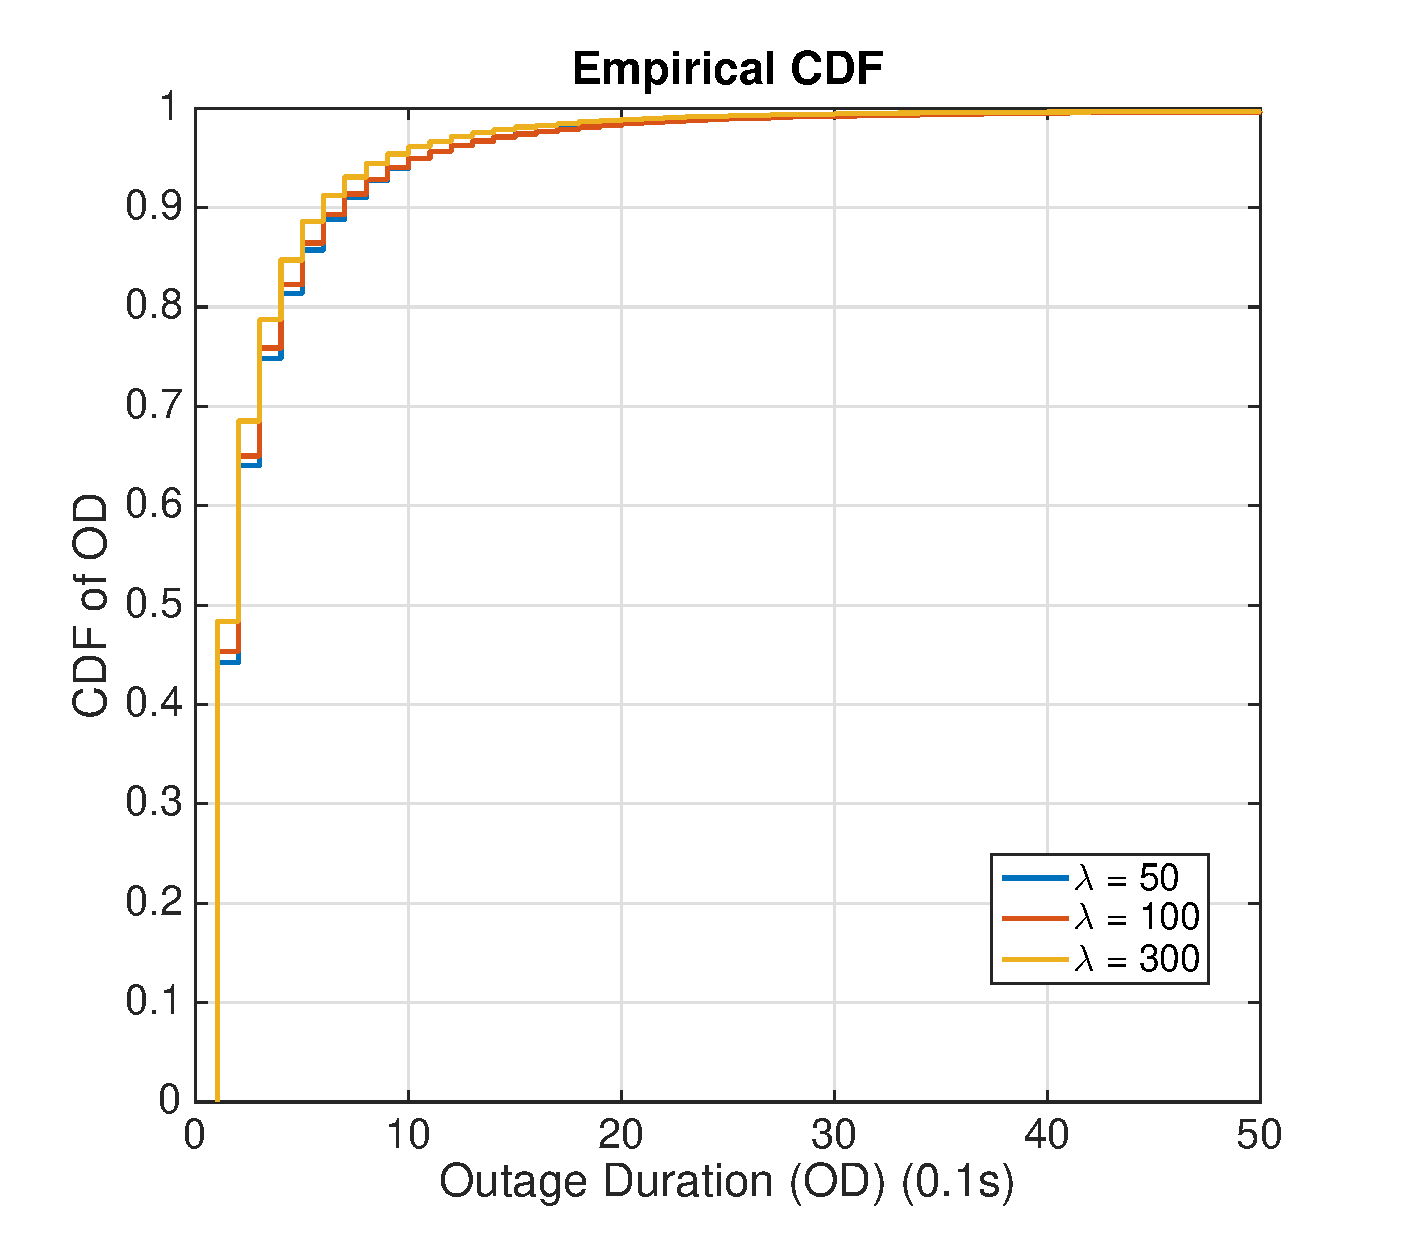
\includegraphics[width=5.5cm]{ODthresh-5DeCorr20MaxMode2.eps}
 %\caption{CDF of Outage Durations when MS is connecting to the Strongest BS with correlated shadowing (de-correlation distance: 200m)}
 \label{corr202}
 }
 \hfil
\subfigure[Correlated shadow fading with $200m$ de-correlation distance]{
 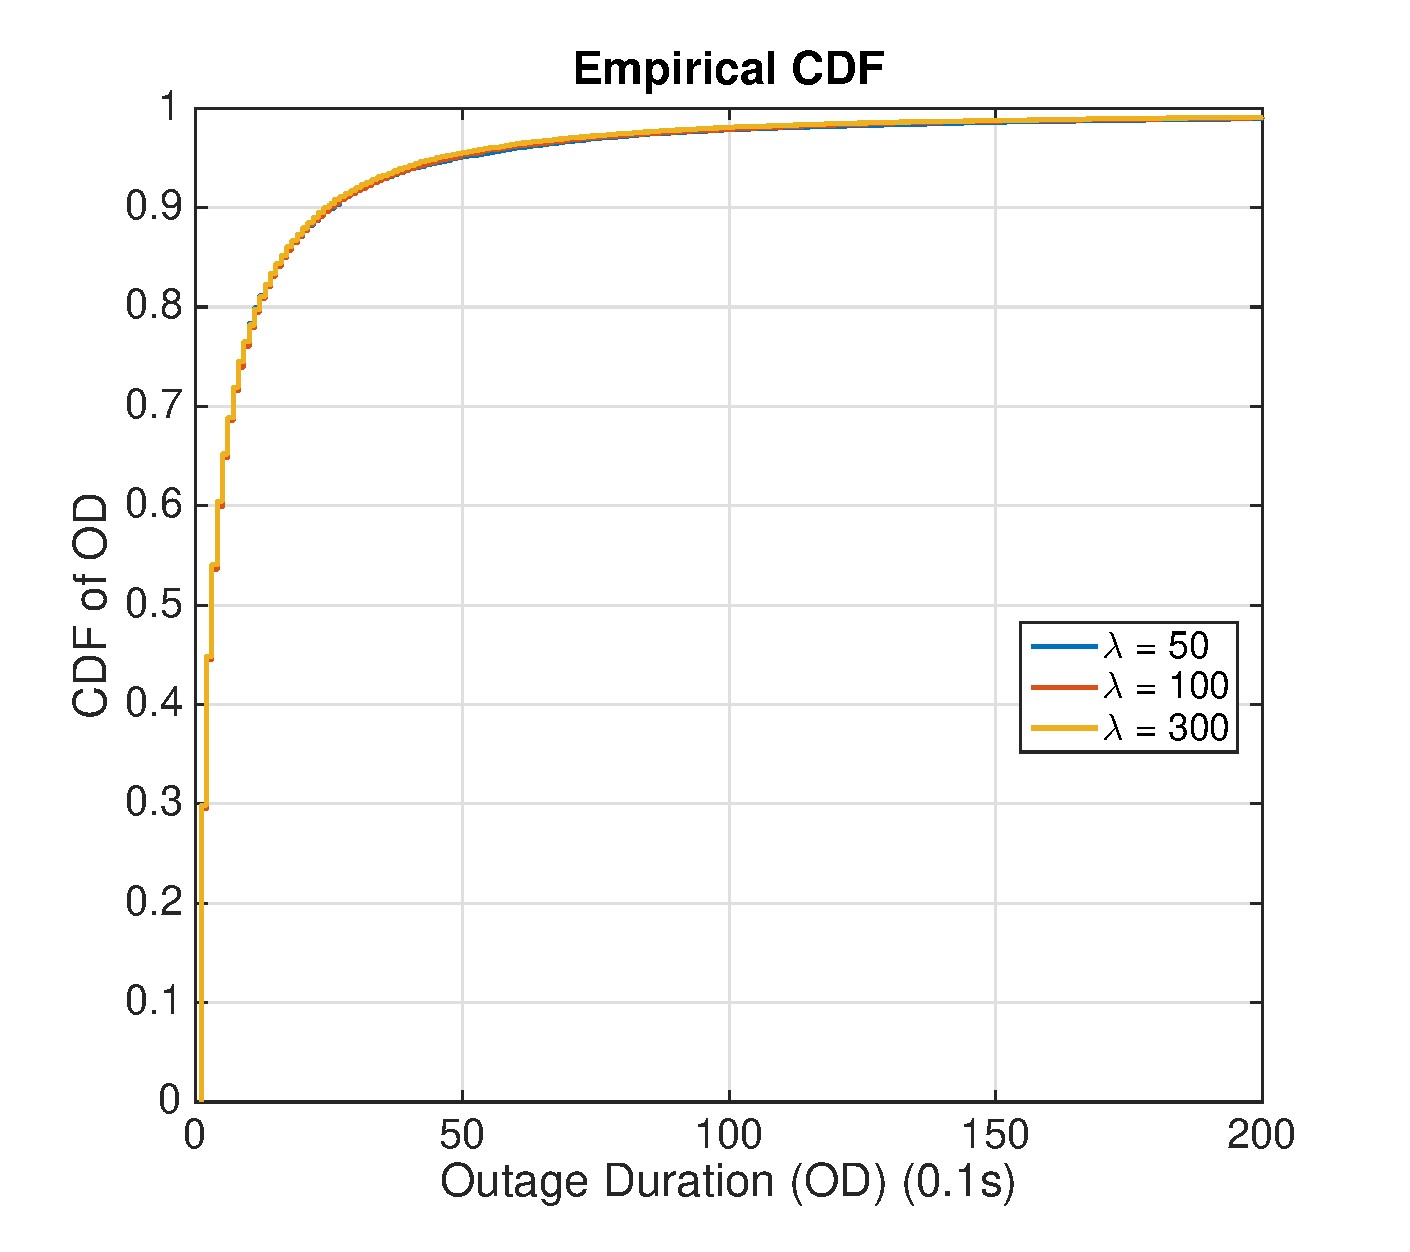
\includegraphics[width=5.5cm]{ODthresh-5DeCorr200MaxMode2.eps}
 %\caption{CDF of Outage Durations when MS is connecting to the Strongest BS with correlated shadowing (de-correlation distance: 200m)}
 \label{corr2002}
 }
 \caption{CDF of Outage Durations when MS is connecting to the Strongest BS with correlated shadowing}
 \label{outageduration1}
 \end{figure*}
 \par Next, we move forward to investigate the system performance when the MS chooses to connect to the BS which provides the highest SINR. The same simulations as done for the nearest BS scenario are executed to explore this scenario. Fig. \ref{strongestBS} presents the receiving SINR of the MS when connecting to the strongest BS. In Fig. \ref{4:Mode12}, \ref{4:Mode22} and \ref{4:Mode32}, the CDF curves of SINR almost overlap each other when increasing BS densities, which means increasing BS density will not change the CDF of SINR significantly. Fig. \ref{fig: outprobs2} shows the outage probability bars, which are consistent with our conclusion. For each shadow fading model, the difference between the highest outage probability and the lowest outage probability is less than $5\%$. Comparing three different shadow fading models, we can conclude that when the MS is connecting to the strongest BS, long de-correlation distance will harm the system performance by increasing the outage probability (yellow bars are higher than green or blue bars). 
 \par Comparing Fig. \ref{fig: outprob1} with Fig. \ref{fig: outprobs2}, we find that with the same BS density, outage probabilities are lower for every shadow fading model if the MS is connecting to the strongest BS. For example, with the independent shadow fading and the BS density being $50$, the outage probability of the Nearest BS mode is $38\%$, while this probability for the Strongest BS mode is $6\%$. For correlated shadow fading with the de-correlation distance being $200m$ and the BS density being $50$, we find that the outage probability of the Nearest BS mode is around $30\%$. This is higher than that of the Strongest BS mode, which is $14\%$. Therefore, we conclude that connecting to the BS which provides highest SINR will improve the system performance for the same network setup. 








 \par In the end, we investigate the system performance from the perspective of outage duration. We use the Random Waypoint mobility model to model the user mobility. The parameters of the Random WayPoint model are given in Table \ref{RWP}. The MS speed is assumed to be between $1m/s$ (pedestrian speed) and $20m/s$ (highway car speed). The MS pause interval is assumed to be uniformly distributed between $0s$ to $60s$. The simulation time slot is set to be $0.1s$, which means we check the MS's SINR every $0.1s$ to determine if it is in the outage area or not. For every simulation scenario, a $50s$ trajectory of the MS is investigated. Simulation results are shown in Fig. \ref{outageduration0} and Fig. \ref{outageduration1}. Comparing Fig. \ref{iid1} with Fig. \ref{corr201} and Fig. \ref{corr2001}, and Fig. \ref{iid2} with Fig. \ref{corr202} and Fig. \ref{corr2002}, we conclude that when the channel is under independent shadow fading, the outage duration is usually less than $2s$. However,  when the channel is under correlated shadow fading with $20m$ de-correlation distance, the outage duration can be longer than $5s$; and when the de-correlation distance is $200m$, the outage duration can be longer than $20s$. Therefore, we draw the conclusion that correlated shadow fading leads to long-lasting outage durations and deteriorates the system performance. Comparing Fig. \ref{iid1} with Fig. \ref{iid2},  Fig. \ref{corr201} with Fig. \ref{corr202}, Fig. \ref{corr2001} with Fig. \ref{corr2002}, we find that connecting to the strongest BS will reduce the outage duration. For example, in Fig. \ref{iid1}, the percentage of outage durations of the Nearest BS mode with a length less than $0.5s$ is $94\%$, while in Fig. \ref{iid2}, that of the Strongest BS mode is $100\%$.  Fig. \ref{corr201} and Fig. \ref{corr202} confirm this conclusion while the percentage of outage durations of the Nearest BS mode with a length less than $5s$ is $95\%$ and that of the Strongest BS mode is $100\%$. In addition, the percentage of outage durations less than $5s$ in Fig. \ref{corr2001} is $85\%$ with BS density being $50$. However, this percentage in Fig. \ref{corr2002} increases to $95\%$. Furthermore, Fig. \ref{corr2001} indicates that increasing the BS density will reduce the percentage of long-lasting outage durations if the MS is connecting to the nearest BS. For example, in Fig. \ref{corr2001}, when the BS density increases from $50$ to $300$, the percentage of outage durations longer than $5s$ is reduced from $15\%$ to $8\%$. In contrast, for independent shadow fading and correlated shadow fading with the MS connecting to the strongest BS, increasing the BS density will not change the distribution of outage durations, which is confirmed by Fig. \ref{iid1}, Fig. \ref{iid2} and Fig. \ref{corr2002}. All CDF curves of outage durations are the same with different BS densities. Comparing Fig. \ref{corr201} and Fig. \ref{corr2001}, Fig. \ref{corr202} and Fig. \ref{corr2002}, we conclude that correlated shadow fading with long de-correlation distance brings long-lasting outage durations. For example, in Fig. \ref{corr2001} with $\lambda = 50$, the percentage of outage durations shorter than $5s$ is $85\%$. However, that percentage is $95\%$ in Fig. \ref{corr201}.
 \begin{table}
 \centering
 \caption{\label{RWP}Random Waypoint Mobility Model Parameters}

 \begin{tabular}{|c|c|}

 \hline
 Speed Interval & $1m/s - 20m/s$\\
 \hline
 Pause Interval & $0s - 60s$\\
 \hline
 Sample Time & $0.1s$\\
 \hline
 \end{tabular}

 \end{table}

 \section{Conclusions}
 \label{Conclusion}
 Shadow fading is large-scale fading, which can cause significant received power loss for a wide area. In general, shadow fading is considered to be independent log-normal distributed to simplify the analysis; however, this is not the real case. In reality, shadow fading at two different positions are correlated to each other. Correlated shadow fading will result in correlated outage events and long-lasting outage durations. To investigate the performance of a multi-cell system given correlated shadow fading, simulations are implemented to analyze the outage probability and the outage duration distribution. First of all, the probability of two different BS layouts: Grid model and Random model are investigated. We find that the Grid model predicts better performance than the Random model. Secondly, outage probabilities given different BS densities and two different connecting strategies: Nearest BS mode and Strongest BS mode, are simulated. We conclude that connecting to the strongest BS will reduce the outage probability compared with the nearest BS from simulation results. Increasing the BS density will not reduce the outage probability when the MS is connecting to the strongest BS. However, when the MS is connecting to the nearest BS and the de-correlation distance of correlated shadow fading is large enough, increasing the BS density will reduce the outage probability.  Finally, we analyze the system performance in terms of outage duration. Simulation results show that correlated shadow fading will result in long-lasting outage durations. Long de-correlation distance brings long-lasting outage durations. Simulation results also show that increasing the BS density will reduce the percentage of long-lasting outage durations if the MS chooses to connect to the nearest BS. Therefore, we suggest dense BS layout might be a proper strategy for next generation mmWave communication networks with correlated shadow fading.

%\appendices
%\section{Proof of the ...}
%Appendix one text goes here.
%
%
%\section{}
%Appendix two text goes here.
%
%
%
%\section*{Acknowledgment}
%
%
%The authors would like to thank...



\ifCLASSOPTIONcaptionsoff
  \newpage
\fi


\bibliography{mybib}

%It is not necessary to upload the biography when you submit your manuscript.
\begin{IEEEbiography}{Tingting Lu}
received her B.S. degree in Automation from University of Science and Technology of China, 
China, in 2008, and her M.S. degree in Electrical Engineering from the Pennsylvania State University, 
State College, in 2010. Currently, she is a Ph.D. candidate in the ECE department at NYU 
Tandon School of Engineering. Her research interests are in analyzing cellular system performance 
under correlated shadow fading for both physical layer and transport layer.
\end{IEEEbiography}
\begin{IEEEbiography}{Pei Liu}
is a research assistant professor in the ECE Department
at NYU Polytechnic School of Engineering. He
received his Ph.D. degree in electrical and computer engineering
from NYU Polytechnic School of Engineering in
2007. He received his B.S. and M.S. degrees in electrical
engineering from Xi'an Jiaotong University, China, in 1997
and 2000, respectively. His research interests are in designing
and analyzing wireless network protocols with an
emphasis on cross-layer optimization, especially for the
PHY and MAC layers.
\end{IEEEbiography}
\begin{IEEEbiography}{SHIVENDRA S. PANWAR}
 is a professor in the ECE Department
at NYU Polytechnic School of Engineering. He is the
director of the New York State Center for Advanced Technology
in Telecommunications (CATT), the faculty director
of the New York City Media Lab, and a member of NYU
Wireless. He co-authored TCP/IP Essentials: A Lab Based
Approach (Cambridge University Press). He was a winner of
the IEEE Communication Society's Leonard Abraham Prize
for 2004.
\end{IEEEbiography}
\end{document}
